\documentclass[numberindividually, numberwithin=section]{hrflecture}
\renewcommand*{\sectionformat}{\textsection\thesection\autodot\enskip}
\addtokomafont{section}{\mdseries}
\let\Mat\relax
\DeclareMathOperator{\Mat}{M}
\let\angleold=\angle
\renewcommand*{\angle}{\sphericalangle}



\subject{Vorlesungsmitschrift}
\title{AGLA \texorpdfstring{\Romannum{2}}{2}}
\subtitle{Prof.~Dr.~Damaris~Schindler}
\date{Auf dem Stand vom \today}
\author{Henry Ruben Fischer}

% \includeonly{lec_07}

\begin{document}
\maketitle

\newpage
\textbf{Disclaimer}
\vspace{1cm}

Nicht von Professor Schindler durchgesehene Mitschrift, keine Garantie auf Richtigkeit ihrerseits.

\newpage
\tableofcontents
\newpage


\automark{section}
% some more adjustments
\makeatletter
\renewtheorem{satz}[lemma]{Satz}
\makeatother

% Begin of lectures
% !TEX root = ./Vorlesungsmitschrift AGLA 2.tex 
\chapter{Affine Geometrie}
\lecture{1}{Di 21.04. 10:15}{}
\section{Was ist ein affiner Raum?}
\begin{beispiel}[aus der AGLA \Romannum{1}]
    \( \reals^2, \reals^3 \). 
    In diesen Räumen gibt es einen ausgezeichneten \enquote{Usprung}.
\end{beispiel}
\begin{frage*}
    Wie könne wir eine affine Ebene / affine Röume modellieren, wobei alle Punkte gleichberechtigt sind?
\end{frage*}
\begin{idee*}
    Verwende affine Unterräume.
\end{idee*}
\begin{beispiel}\label{affiner_unterraum}
    Sei \( K \) ein Körper, \( V \) ein \( K \)-Vektorraum, \( W\subseteq V \) ein Untervektorraum und \( v\in V \). 
    Wir nennen \( X=v+W \) einen affinen Unterraum von \( V \). 
    \( X \) ist im Allgemeinen selbst kein Vektorraum unter der Addition in \( V \), aber \( W \) \enquote{operiert} auf \( X \).
    \begin{figure}[H]
        \centering
        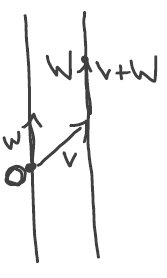
\includegraphics[width=0.2\linewidth]{figures/affiner_unterraum}
        \label{fig:affiner_unterraum}
    \end{figure}
    
    Für \( w\in W \) definieren wir die Abbildung
    \begin{align*}
        \tau_w\maps \begin{aligned}[t] 
            X&\to X\\
            p &\mapsto p+w.
        \end{aligned}
    \end{align*}
    \begin{figure}[H]
        \centering
        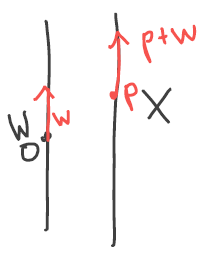
\includegraphics[width=0.2\linewidth]{figures/tau_w}
        \label{fig:tau_w}
    \end{figure}
    Sei
    \begin{align*}
        \Bij(X)=\Set{f\maps X\to X, f \text{ ist bijektiv}}.
    \end{align*}
    Dann ist \( \tau_w\in \Bij(X) \) für alle \( w\in W \).
\end{beispiel}
\begin{bemerkung*}
    \( \Bij(X) \) ist eine Gruppe unter Verkettung von Abbildung. 
    Wir erhalten eine Abbildung
    \begin{align*}
        \tau\maps \begin{aligned}[t] 
            W &\to \Bij(X)\\
            w &\mapsto \tau_w.
        \end{aligned}
    \end{align*}
\end{bemerkung*}
\begin{lemma}
    Die Abbildung \( \tau \) ist ein Gruppenhomomorphismus.
\end{lemma}
\begin{proof}
    Seien \( w, w' \in W \)
    Dann
    \begin{align*}
        \tau_w\circ \tau_{w'}\maps \begin{aligned}[t] 
            X &\to X\\
            p &\mapsto p+\underbracket{w'+w},
        \end{aligned}
    \end{align*}
    also
    \begin{align*}
        \tau(w)\circ \tau(w')=\tau_w\circ \tau_{w'}=\tau_{w+w'}=\tau(w+w').
    \end{align*}
    
\end{proof}
Es gilt noch mehr:

\textcolor{Turquoise}{für \( p, q \in X \)} besteht genau ein \( w\in W \) mit \( \tau_w(p)=q \).

\begin{figure}[H]
    \centering
    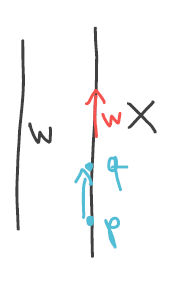
\includegraphics[width=0.2\linewidth]{figures/tau_w_bijektion}
    \label{fig:tau_w_bijektion}
\end{figure}

\section*{Gruppenoperationen}
\begin{beispiel}\label{d_3}
    Betrachte ein gleichseitiges Dreieck \( D \) und Spiegelungen / Drehungen die \( D \) auf sich selbst abbilden.

    \begin{figure}[H]
        \centering
        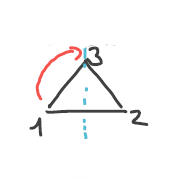
\includegraphics[width=0.2\linewidth]{figures/d_3}
        \label{fig:d_3}
    \end{figure}
    Diese formen eine Gruppe (welche?) und \enquote{operieren} auf \( D \).
\end{beispiel}
\begin{definition}
    Sei \( X \) eine Mege und \( G \) eine Gruppe. 
    Eine Operation von \( G \) auf \( X \) ist ein Homomorphismus von Gruppen
    \begin{align*}
        \tau\maps \begin{aligned}[t] 
            G&\to \Bij(X)\\
            g&\mapsto \tau_g.
        \end{aligned}
    \end{align*}
\end{definition}
\begin{bemerkung*}
    \( \tau \) ist ein Homomorphismus \dh \tforall \( g, g' \in G \)
    \begin{align*}
        \tau_g\circ \tau_{g'}=\tau_{gg'}.
    \end{align*}
    
    Für \( x\in X \) nennen wir
    \begin{align*}
        G(x)=\Set{\tau_g(x)|g\in G}
    \end{align*}
    die Bahn von \( x \) unter \( G \).
\end{bemerkung*}
\begin{beispiel}\label{operation:beispiele}
    \begin{eigenschaftenenumerate}
        \item \label{operation:beispiele:linkstranslation} Sei \( G \) eine Gruppe und \( X=G \) die Linkstranslation \( l\maps \begin{aligned}[t] 
            G&\to \Bij(G)\\
            g&\mapsto l_g
        \end{aligned} \) mit \( l_g(x)=gx \quad\forall x\in G \) ist eine Gruppenoperation von \( G \) auf sich selbst.
        
        \item \label{operation:beispiele:konjugation}\begin{align*}
            k\maps \begin{aligned}[t] 
                G &\to \Bij(G)\\
                g &\mapsto kg
            \end{aligned}
        \end{align*}
        mit \( k_g(x)=gx\inv{g} \quad\forall x\in G \) ist eine Gruppenoperation.
    \end{eigenschaftenenumerate}
\end{beispiel}
\thref{operation:beispiele}~\ref{operation:beispiele:konjugation}
\begin{frage*}
    Sei \( \tau\maps G\to \Bij(x) \) eine Gruppenoperation, \( x,y\in X \). 
    Wann gibt es ein \( g\in G \) mit \( \tau_g(x)=y \)?
    \begin{figure}[H]
        \centering
        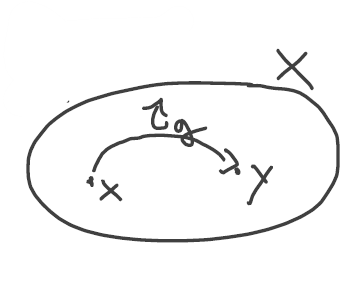
\includegraphics[width=0.5\linewidth]{figures/einfach_transitiv}
        \label{fig:einfach_transitiv}
    \end{figure}
    
\end{frage*}

\begin{definition*}
    Sei \( \tau\maps G\to \Bij(X) \) eine Gruppenoperation von \( G \) auf \( X \). 
    Wir nennen \( \tau \) \emph{einfach transitiv}, wenn \tforall \( x,y\in X \) \emph{genau ein} \( g\in G \) besteht mit
    \begin{align*}
        \tau_g(x)=y.
    \end{align*}
\end{definition*}
\begin{beispiel*}
    \begin{itemize}
        \item Die Gruppenoperation aus \thref{d_3} ist \emph{nicht} einfach transitiv
        \begin{figure}[H]
            \centering
            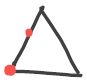
\includegraphics[width=0.2\linewidth]{figures/d_3_nicht_einfach_transitiv}
            \label{fig:d_3_nicht_einfach_transitiv}
        \end{figure}
        
        \item Die Linkstranslation aus \thref{operation:beispiele}~\ref{operation:beispiele:linkstranslation} ist immer einfach transitiv.
    \end{itemize}
\end{beispiel*}
Zurück zum \thref{affiner_unterraum} (\( V \) \( K \)-Vektorraum, \( W\subseteq V \) Untervektorraum, \( v\in V \), \( X=v+W \))

Wir haben Translationen definiert
\begin{align*}
    \tau\maps \begin{aligned}[t] 
        W&\to \Bij(X)\\
        x&\mapsto \tau_w
    \end{aligned}
\end{align*}
mit \( \tau_w\maps X\to X \), \( p\mapsto p+w \). 
\( \tau \) ist eine einfach transitive Gruppenoperation von \( W \) auf \( x \).

\begin{figure}[H]
    \centering
    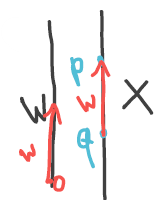
\includegraphics[width=0.2\linewidth]{figures/affiner_unterraum_einfach_transitive_gruppenoperation}
    \label{fig:affiner_unterraum_einfach_transitive_gruppenoperation}
\end{figure}

\begin{definition*}
    Sei \( K \) ein Körpr. 
    Ein affiner Raum über \( K \) ist ein Tripel \( (X, T(X), \tau ) \) mit
    \begin{itemize}
        \item \( X\neq \emptyset \) eine Menge 
        \item \( T(X) \) ein \( K \)-Vektorraum 
        \item \( \tau\maps T(x)\to \Bij(X) \) eine einfach transitive Gruppenoperation
    \end{itemize}
\end{definition*}
\begin{konvention*}
    \( X=\emptyset \) ohne Spezifikation von \( T(X) \), \( \tau \) nennen wir auch einen affinen Raum.
\end{konvention*}
\begin{figure}[H]
    \centering
    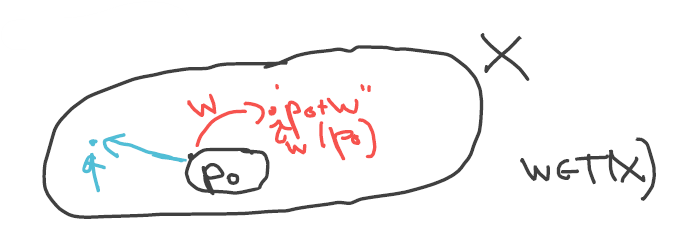
\includegraphics[width=0.5\linewidth]{figures/affiner_raum}
    \label{fig:affiner_raum}
\end{figure}
\begin{definition*}
    Sei \( (X,T(X),\tau) \) in affiner Raum über einem Körper \( K \). 
    Dann nennen wir \( \dim_K T(X) \) die Dimension von \( X \), schreiben auch \( \dim X \).
     
    Ist \( \dim X=1 \) \bzw \( \dim X=2 \), dann nennen wir \( X \) eine affine Gerade \bzw affine Ebene.
\end{definition*}

Sei \( (X, T(X), \tau) \) in affiner Raum, \( p,q\in X \). Dann \( \existsone t\in T(X) \) mit \( \tau_t(p)=q \).

\textcolor{Turquoise}{Schreibe \( \vv{pq}=t\in T(X) \) als \( \tau_{\vv{pq}}(p)=q \).}
\begin{figure}[H]
    \centering
    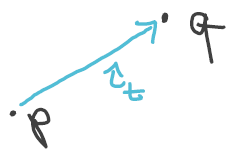
\includegraphics[width=0.2\linewidth]{figures/vektornotation}
    \label{fig:vektornotation}
\end{figure}
Wir erhalten eine Abbildung
\begin{align*}
    X\times X&\to T(X)\\
    (p,q)&\mapsto \vv{pq}.
\end{align*}
\begin{frage*}
    Welche Eigenschaften hat die Abbildung \( (p,q)\mapsto \vv{pq} \) in einem allgemeinen affinen Raum?
\end{frage*}
\begin{lemma}\label{vektoren_funzen_richtig}
    Sei \( X \) ein affiner Raum, \( p,q,r\in X \). Dann gilt \( \vv{pq}+\vv{qr}=\vv{pr} \).
\end{lemma}
\begin{figure}[H]
    \centering
    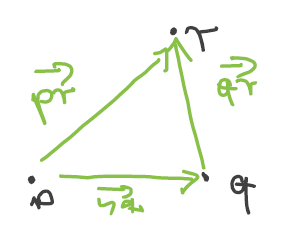
\includegraphics[width=0.3\linewidth]{figures/vektoren_funzen_richtig}
    \label{fig:vektoren_funzen_richtig}
\end{figure}
\begin{proof}
    \( \tau\maps T(X)\to \Bij(X) \) ist ein Homomorphismus. 
    Also gilt \( \tau_{\vv{qr}}\circ \tau_{\vv{pq}}=\tau_{\vv{pq}+\vv{qr}} \). 
    Es gilt damit \( \tau_{\vv{pq}+\vv{qr}}(p)=r \). 
    Also \( \vv{pq}+\vv{qr}=\vv{pr} \).    
\end{proof}

\section{Affine Abbildungen}
Seien \( V,W \) \( K \)-Vektorräume.
In der AGLA \Romannum{1}: lineare Abbildungen
\begin{align*}
    F\maps V\to W,
\end{align*}
\dh \( F \) respektiert die Vektorraum-Struktur
\begin{align*}
    F(v_1+v_2)=F(v_1)+F(v_2)\quad\forall v_1,v_2\in V\\
    F(\lambda v)=\lambda F(v)\quad \forall\lambda\in K \forall v \in V.
\end{align*}
\begin{frage*}
    Was sind natürliche Abbildungen zwischen affinen Räumen?
\end{frage*}
Seien \( X, Y \) affine Räume über einem Körper \( K \).

Seien \( X, Y \) affine Räume über einem Körper \( K \)
\begin{figure}[H]
    \centering
    \includegraphics[width=0.8\linewidth]{figures/affine_Abbildungen}
    \label{fig:affine_Abbildungen}
\end{figure}
\begin{align*}
    \textcolor{Turquoise}{\vertrelate{\vertni}{T(X)}{\vv{pq}}\rightsquigarrow\vertrelate{\vertni}{T(Y)}{\vv{f(p)f(q)}}}.
\end{align*}
\begin{definition*}
    Wir nennen eine Abbildung \( f\maps X \to Y \) affin, wenn s eine \( K \)-lineare Abbildung \( F\maps T(X)\to T(Y) \) gibt, sodass \tforall \( p,q\in X \) gilt
    \begin{align*}
        \vv{f(p)f(q)}=F(\vv{pq}).
    \end{align*}
\end{definition*}
\begin{bemerkung*}
    \begin{eigenschaftenenumerate}
        \item Es gibt im Allgemeinen verschiedene affine Abbildungen \( f\maps X \to Y \), die zur gleichen linearen Abbildung \( F\maps T(X)\to T(Y) \) gehören.
        \item Sei \( p_0 \in X \) fest und \( f\maps X \to Y \) affin.
        
        Für \( q\in X \) gilt
        \begin{align*}
            f(q)\begin{aligned}[t] 
                &=\tau_{\vv{f(p_0)f(q)}}(f(p0))\\
            &=\tau_{F(\vv{p_0 q})}(f(p0)).
            \end{aligned}
        \end{align*}
        Also bestimmen \( f(p_0) \) und \( F \) zusammenen die Abbildung \( f\maps X\to Y \).
    \end{eigenschaftenenumerate}


\end{bemerkung*}
\begin{beispiel*}
    Seien \( V,W \) \( K \)-Vektorräume
    \begin{align*}
        X=(V,V,\tau),\quad Y=(W,W,\tau).
    \end{align*}
    Eine affine Abbildung \( f\maps V\to W \) ist eindeutig bestimmt durch \( f(0) \) und eine lineare Abbildung \( F\maps V\to W \). Es gilt
    \begin{align*}
        f(v)=\textcolor{Goldenrod}{f(0)}+\textcolor{LimeGreen}{F(v)}\quad\forall \textcolor{LimeGreen}{v} \in V.
    \end{align*}
\end{beispiel*}
\begin{figure}[H]
    \centering
    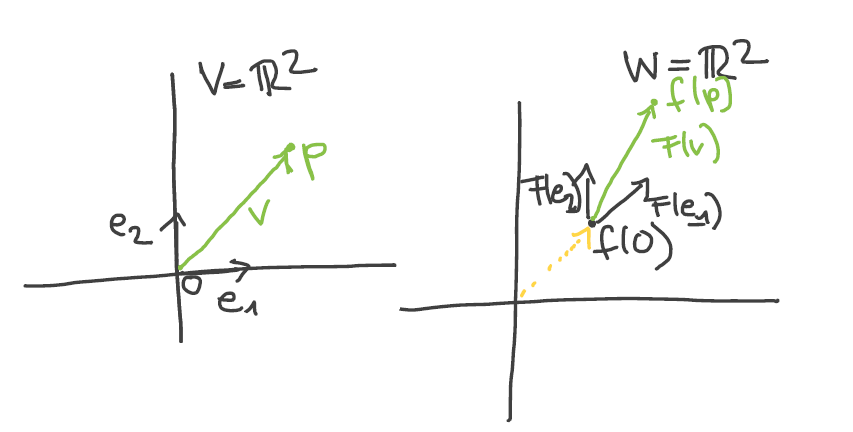
\includegraphics[width=0.7\linewidth]{figures/affine_abbildungen_vektorraeume}
    \label{fig:affine_abbildungen_vektorraeume}
\end{figure}
\begin{bemuebung*}
    Eine affine Abbildung \( f\maps X \to Y \) ist genau dann injektiv \bzw surjektiv \bzw bijektiv, wenn die zugehörige Abbildung \( F\maps T(X)\to T(Y) \).
\end{bemuebung*}
\begin{definition*}
    Wir nennen eine bijektive affine Abbildung \( f\maps X \to Y \) eine Affinität.
\end{definition*}
\section*{Affine Unterräume}
\begin{beispiel*}[\( \reals^2 \) als Vektorraum.]
    Untervektorräume von \( \reals^2 \) sind \( \emptyset \), \( \zeroset \), \( \reals^2 \) und Geraden durch \( 0 \).
    \begin{figure}[H]
        \centering
        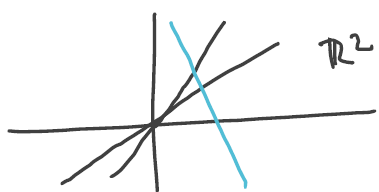
\includegraphics[width=0.4\linewidth]{figures/untervektorraeume_r2}
        \label{fig:untervektorraeume_r2}
    \end{figure}
    Betrachte nun \( \reals^2 \) als affinen Raum.
    \begin{figure}[H]
        \centering
        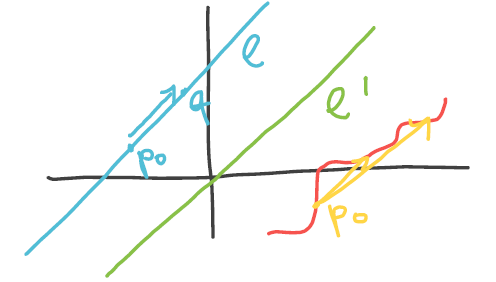
\includegraphics[width=0.5\linewidth]{figures/affine_unterraeume_r2}
        \label{fig:affine_unterraeume_r2}
    \end{figure}
    \begin{idee*}
        Wir wollen \( l \) und \( l' \) als affine Unterräume von \( \reals^2 \) definieren, da die Verschiebung von \( l, l' \) jeweils Untervektorräume von \( \reals^2 \) sind.
    \end{idee*}
\end{beispiel*}

\begin{definition*}
    Sei \( (X,T(X), \tau) \) in affiner Raum und \( Y\subseteq X \). Wenn es einen Punkt \( p_0 \in Y \) gibt, sodass
    \begin{align*}
        T(Y)\definedas \Set{\vv{p\circ q}\in T(X), q\in Y}
    \end{align*}
    ein Untervektorraum von \( T(X) \) ist, dann nennen wir \( Y \) einen affinen Unterraum von \( X \).
\end{definition*}
\begin{lemma}
    Sei \( Y\subseteq X \) ein affiner Unterraum eines affinen Raumes \( (X,T(X),\tau) \). Dann gilt
    \begin{align*}
        T(Y)=\Set{\vv{pq}\in T(X), q\in Y}
    \end{align*}
    für jedes beiliebigen Punkt \( p\in Y \).
\end{lemma}
\begin{proof}
    Sei \( p_0\in Y \) ein fester Punkt mit
    \begin{align*}
        T(Y)=\Set{\vv{p_0 q}\in T(X), q \in Y}
    \end{align*}
    Untervektorraum von \( T(X) \).
    Dann gilt für \( p \in Y \)
    \begin{align*}
        \Set{\vv{pq}|q\in Y}=\vv{pp_0}+\Set{\vv{p_0 q}| q\in Y}=\vertrelate{\vertni}{T(Y)}{\vv{p p_0}}+ T(Y)=T(Y),
    \end{align*}
    da \( \vv{p p_0}=-\vv{p_0 p}\in T(Y) \).
    
\end{proof}
\begin{definition*}
    Sei \( Y\subseteq X \) ein affiner Unterraum. Wir nennen \( \dim_K T(Y) \) die Dimension von \( Y \) und schreiben 
    \begin{align*}
        \dim Y=\dim_K T(Y).
    \end{align*}
\end{definition*}



% !TEX root = ./Vorlesungsmitschrift AGLA 2.tex  
\lecture{Fr 24.10. 10:15}{}
\section{Durchschnitt und Verbindung affiner Räume}
\begin{frage*}
    Sei \( X \) ein affiner Raum, \(    Y_1, Y_2 \) affine Unterräume von \( X \). Sind \( Y_1\cap Y_2, Y_1\cup Y_2 \) auch affine Unterräume von \( X \)?
    \begin{figure}[H]
        \centering
        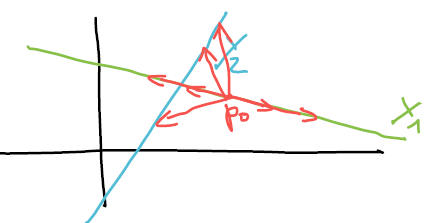
\includegraphics[width=0.5\linewidth]{figures/verbindung_affine_raeume}
        \caption*{\( X=\reals^2 \)}
        \label{fig:verbindung_affine_raeume}
    \end{figure}
\end{frage*}
\begin{lemma}\label{schnittraum:translationen}
    Sei \( X \) ein affiner Raum, \( Y_i \), \( i\in I \), eine Familie von affinen Unterräumen von \( X \).

    Dann ist \( Y\definedas \bigcap_{i\in I} Y_i \) ein affiner Unterraum von \( X \).

    Wenn \( Y\neq \emptyset \), dann gilt
    \begin{align*}
        T(Y)=\bigcap_{i\in I}T(Y_i).
    \end{align*}
\end{lemma}
\begin{proof}
    Falls \( Y=\emptyset \): \checkmark

    Wir nehmen also an \( Y\neq \emptyset \).
    Sei \( p_0\in Y \).
    Dann gilt:
    \begin{align*}
        T(Y)\begin{aligned}[t] 
            &=\Set{\underrelate{\textcolor{Goldenrod}\vertni}{\textcolor{Goldenrod}{T(X)}}{\vv{p_0 q}},q\in \bigcap_{i\in I}Y_i}\\
            &=\bigcap_{i\in I}\textcolor{LimeGreen}{\underbrace{\Set{\vv{p_0 q}, q\in Y_i}}_{=T(Y_i)}}\\
            &=\bigcap_{i\in I}T(\explain[big]{\text{Untervektorräume von \( T(X) \)}}{Y_i}).
        \end{aligned}
    \end{align*}
    Also ist \( T(Y) \) ein Untervektorraum von \( T(X) \) und \( T(Y)=\bigcap_{i\in I}T(Y_i) \).
\end{proof}
\begin{bemerkung*}
    In obiger Notation ist \( \bigcup_{i\in I}Y_i \) im Allgemeinen kein affiner Unterraum von \( X \).
\end{bemerkung*}
\begin{frage*}
    Finde den \enquote{kleinsten} affinen Unterraum von \( X \), der \( \bigcup_{i\in I}Y_i \) enthält! (\zb \( X\supseteq \bigcup_{i\in I} Y_i\), aber \( X \) ist im Allgemeinen nicht \enquote{minimal}).
\end{frage*}
\begin{definition*}
    Sei \( X \) ein affiner Raum, \( Y_i \), \( i\in I \) affine Unterräume von \( X \). Wir nennen
    \begin{align*}
        \bigcap_{\mathclap{\substack{Y\subseteq X \text{ aff.\ Unterraum}\\
         \bigcup_{i\in I}Y_i\subseteq Y}}}Y
    \end{align*}
    den \emph{Verbindungsraum} der affinen Unterräume \( Y_i \), \( i\in I \). Schreibe \( \bigvee_{i\in I}Y_i \).
\end{definition*}
\begin{beispiel*}
    \begin{figure}[H]
        \centering
        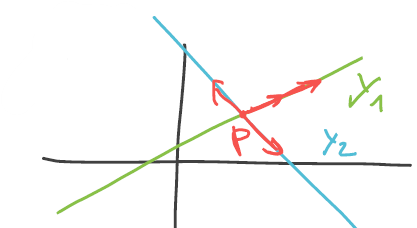
\includegraphics[width=0.5\linewidth]{figures/verbindungsraum_zwei_geraden}
        \caption*{\( X=\reals^2 \), \( Y_1\vee Y_2=X \), \textcolor{OrangeRed}{\( Y=Y_1\vee Y_2 \), \( T(Y)=T(Y_1)+T(Y_2) \)}.}
        \label{fig:verbindungsraum_zwei_geraden}
    \end{figure}
    
\end{beispiel*}

\begin{frage*}
    Wie kann man im Allgemeinen \( T(Y_1\vee Y_2) \) aus \( T(Y_1),T(Y_2) \) bestimmen?
\end{frage*}
\begin{lemma}\label{verbindungsraum:translationen}
    Sei \( X \) ein affiner Raum, \( Y_1,Y_2\neq\emptyset \) affine Unterräume von \( X \).
    \begin{eigenschaftenenumerate}
        \item \label{verbindungsraum:translationen:schnitt_nicht_leer}Sei \( Y_1\cap Y_2\neq \emptyset \).
        Dann gilt
        \begin{align*}
            T(Y_1\vee Y_2)=T(Y_1)+T(Y_2).
        \end{align*}
        
        \item \label{verbindungsraum:translationen:schnitt_leer}Sei \( Y_1\cap Y_2=\emptyset \), \( p_1\in Y_1, p_2\in Y_2\) und \( Y=p_1\vee p_2 \).
        
        Dann gilt:
        \begin{align*}
            T(Y_1\vee Y_2)=(T(Y_1)+T(Y_2))\oplus T(Y).
        \end{align*}
    \end{eigenschaftenenumerate}
\end{lemma}
\begin{proof}
    \begin{proofdescription}
        
        \item[\ref{verbindungsraum:translationen:schnitt_nicht_leer}]
        \begin{figure}[H]
            \centering
            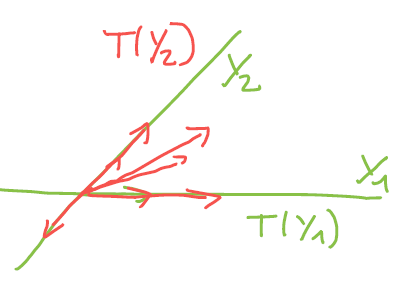
\includegraphics[width=0.5\linewidth]{figures/verbindungsraum_translationen_schnitt_nicht_leer}
            \label{fig:verbindungsraum_translationen_schnitt_nicht_leer}
        \end{figure}
         Sei \( p\in Y_1\cap Y_2 \). Dann gilt
         \begin{align*}
             T(Y_1)\cup T(Y_2)\begin{aligned}[t] 
                &=\Set{\vv{pq}|q\in Y_1\cup Y_2}\\
                &\subseteq T(Y_1\vee Y_2),
             \end{aligned}
         \end{align*}
         also \( T(Y_1)+T(Y_2)\subseteq T(Y_1\vee Y_2) \).

         Sei \( Y=\Set{\tau_t(p)|t\in T(Y_1)+T(Y_2)} \).
         Dann ist \( Y \) affiner Unterraum von \( X \) mit \( Y_1\cup Y_2\subseteq Y \), also \( Y_1\vee Y_2\subset Y \), also \( Y_1\vee Y_2\subseteq Y \). Also gilt
         \begin{align*}
             T(Y_1\vee Y_2)\subseteq T(Y)=T(Y_1)+T(Y_2).
         \end{align*}
         
         Also \( T(Y_1\vee Y_2)=T(Y_1)+T(Y_2) \).
         
         \item[\ref{verbindungsraum:translationen:schnitt_leer}]
         \( Y_1\cap Y_2=\emptyset \), \( p_1\in Y_1 \), \( p_2\in Y_2 \), \( Y=p_1\vee p_2 \).
         \begin{figure}[H]
             \centering
             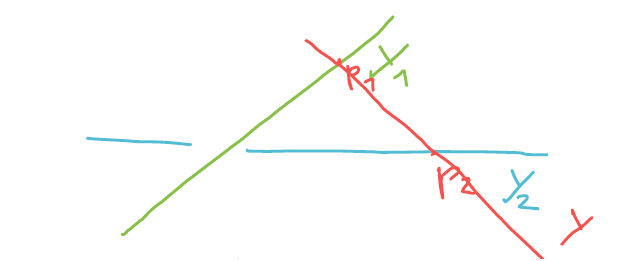
\includegraphics[width=0.5\linewidth]{figures/verbindungsraum_translationen_schnitt_leer}
             \label{fig:verbindungsraum_translationen_schnitt_leer}
         \end{figure}
         Schreibe \( Y_1\vee Y_2=Y_1\vee Y\vee Y_2 \) (verwende dazu \( Y\subseteq Y_1\vee Y_2 \)).
         Verwende \ref{verbindungsraum:translationen:schnitt_nicht_leer} und leite ab, dass gilt:
         \begin{align*}
             T(Y_1\vee Y \vee Y_2)\begin{aligned}[t] 
                 &=T(Y_1)+T(Y\vee Y_2)\\
                 &=T(Y_1)+T(Y)+T(Y_2)\\
                 &=(T(Y_1)+T(Y_2))\needed{\oplus} T(Y).
             \end{aligned}
         \end{align*}
         Es gilt 
         \begin{align*}
             T(Y)=\Set{\lambda\vv{p_1 p_2}| \lambda\in K}.
         \end{align*}
         Wir wollen zeigen
         \begin{align*}
             (T(Y_1)+T(Y_2))\cap T(Y)=\zeroset.
         \end{align*}
         Es genügt zu zeigen
         \begin{align*}
             \vv{p_1 p_2}\notin T(Y_1)+T(Y_2).
         \end{align*}
         Gegenannahme:
         \begin{align*}
             \vv{p_1 p_2}=\underrelate{\vertni}{T(Y_1)}{\vv{p_1 y_1}}+\underrelate{\vertni}{T(Y_2)}{\vv{q_2 p_2}}
         \end{align*}
         mit \( q_1\in Y_1 \), \( q_2\in Y_2 \).
         \begin{figure}[H]
             \centering
             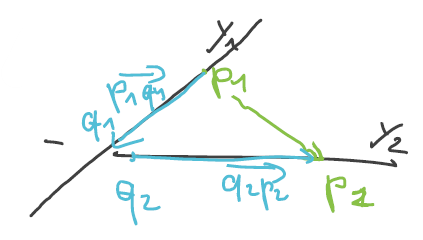
\includegraphics[width=0.5\linewidth]{figures/verbindungsraum_translationen_schnitt_leer_verbindungslinie_nicht_in_translationen}
             \label{fig:verbindungsraum_translationen_schnitt_leer_verbindungslinie_nicht_in_translationen}
         \end{figure}
         Dann gilt
         \begin{align*}
             \vv{q_1 q_2}=\vv{q_1 p_1}+\vv{p_1 p_2}+\vv{p_2 q_2}=0,
         \end{align*}
         also \( q_1=q_2 \) und \( Y_1\cap Y_2\neq \emptyset \) \contra.
    \end{proofdescription}
\end{proof}
Als nächstes: \( \dim(Y_1\vee Y_2) \) ist durch \( \dim_K T(Y_1\vee Y_2) \) gegeben, also sollten wir aus \thref{verbindungsraum:translationen} für \( Y_1\vee Y_2 \) ableiten können.
\begin{lemma}\label{verbindungsraum:dimension}
    Sei \( X \) ein affiner Raum, \( Y_1, Y_2\neq \emptyset \) affine Unterräume von \( X \).
    \begin{eigenschaftenenumerate}
        \item\label{verbindungsraum:dimension:schnitt_nicht_leer} Sei \( Y_1\cap Y_2\neq \emptyset \).
         Dann gilt \( \dim(Y_1\vee Y_2)=\dim(Y_1)+\dim(Y_2)-\dim(Y_1\cap Y_2) \).
        \item\label{verbindungsraum:dimension:schnitt_leer} Sei \( Y_1\cap Y_2=\emptyset \).
        Dann gilt
        \begin{align*}
            \dim(Y_1\vee Y_2)=\dim(Y_1)+\dim(Y_2)-\dim(T(Y_1)\cap T(Y_2))+1.
        \end{align*}
    \end{eigenschaftenenumerate}
    
\end{lemma}
\begin{proof}
    \begin{proofdescription}
        
        \item[\ref{verbindungsraum:dimension:schnitt_nicht_leer}] Aus \thref{verbindungsraum:translationen} folgt
        \begin{align*}
            T(Y_1\vee Y_2)=T(Y_1)+T(Y_2),
        \end{align*}
        aus der Dimensionsformel für Untervektorräume folgt
        \begin{equation*}
            \dim (Y_1\vee Y_2)\begin{aligned}[t] 
                &=\dim T(Y_1\vee Y_2)\\
                &=\dim(Y_1)+\dim T(Y_2)-\dim(T(Y_1)\cap T(Y_2))\\
                &\explain{\text{\thref{schnittraum:translationen}}}{=}\dim T(Y_1)+\dim T(Y_2)-\dim T(Y_1\cap Y_2)\\
                &=\dim Y_1+\dim Y_2-\dim Y_1\cap Y_2.
            \end{aligned}
        \end{equation*}
        
        \item[\ref{verbindungsraum:dimension:schnitt_leer}] \( Y_1\cap Y_2 \), \( p_1\in Y_1 \), \( p_2\in Y_2 \), \( Y=p_1\vee p_2 \).
        
        Dann ist
        \begin{align*}
            \dim Y=\dim T(Y)=1.
        \end{align*}
        Wir erhalten
        \begin{align*}
            \dim (Y_1\vee Y_2)\begin{aligned}[t] 
                &=\dim T(Y_1\vee Y_2)\\
                &\explain{\text{\thref{verbindungsraum:translationen}}}{=}\dim((T(Y_1)+T(Y_2))\oplus T(Y))\\
                &=\dim(T(Y_1)+T(Y_2))+\equalto{1}\dim T(Y)\\
                &=\dim T(Y_1)+\dim T(Y_2)- \dim (T(Y_1)\cap T(Y_2))+1\\
                &=\dim Y_1+\dim Y_2 -\dim(T(Y_1)\cap T(Y_2))+1
            \end{aligned}
        \end{align*}
    \end{proofdescription}
\end{proof}
\begin{beispiel*}[\( X=\reals^3 \)]
    \begin{figure}[H]
        \centering
        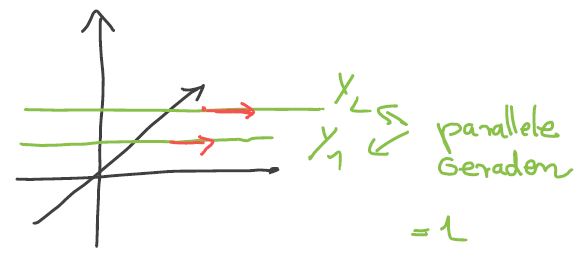
\includegraphics[width=0.5\linewidth]{figures/verbindungsraum_parallele_geraden}
        \label{fig:verbindungsraum_parallele_geraden}
    \end{figure}
    \begin{align*}
        \dim (Y_1\vee Y_2)=1+1-\underbrace{\dim(T(Y_1)\cap T(Y_2))}_{=1}+1=2
    \end{align*}
    \begin{figure}[H]
        \centering
        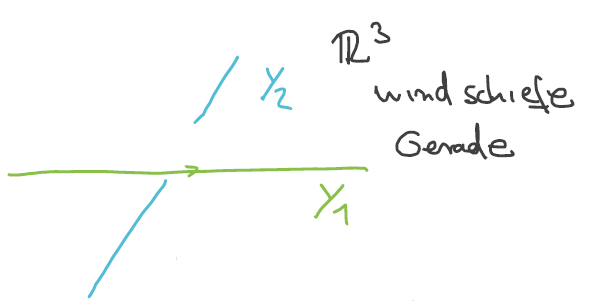
\includegraphics[width=0.6\linewidth]{figures/verbindungsraum_windschiefe_geraden}
        \label{fig:verbindungsraum_windschiefe_geraden}
    \end{figure}
    \begin{align*}
        \dim (Y_1\vee Y_2)1+1-0+1=3
    \end{align*}
    und \( Y_1\vee Y_2=X \).
    
\end{beispiel*}
\section{Parallelprojektionen}
\begin{wiederholung*}[Projektionen aus der \agla{1}]
    \begin{beispiel*}
        \begin{figure}[H]
            \centering
            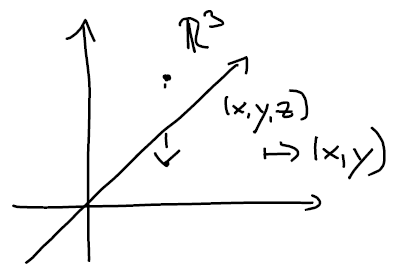
\includegraphics[width=0.5\linewidth]{figures/r_3_projektion}
            \label{fig:r_3_projektion}
        \end{figure}
        
    \end{beispiel*}
    Sei \( V \) ein \( K \)-Vektorraum, \( W, W_1\subset V \) \( K \)-Untervektorräume mit \( V=W\oplus W_1 \).
    Schreibe \( v\in V \) in der Form \( v=w+w_1 \) und mit \( w\in W \), \( w_1\in W_1 \). Definiere
    \begin{align*}
        P_W\maps \begin{aligned}[t] 
            V&\to W_1\\
            \equalto{w+w_1}{v}&\mapsto w_1.
        \end{aligned}
    \end{align*}
    Ein paar Eigenschaften von \( P_W \):
    \begin{itemize}
        \item \( P_W\maps V \to W_1 \) ist eine lineare Abbildung,
        \item \( \Ker P_W=W \),
        \item \( \evaluateat{P_W}{W_1}=\Id_{W_1} \).
    \end{itemize}
    Als Nächstes:
    Wir schränken \( P_W \) ein auf einen Untervektorraum \( W_0 \) von \( V \).
    \begin{figure}[H]
        \centering
        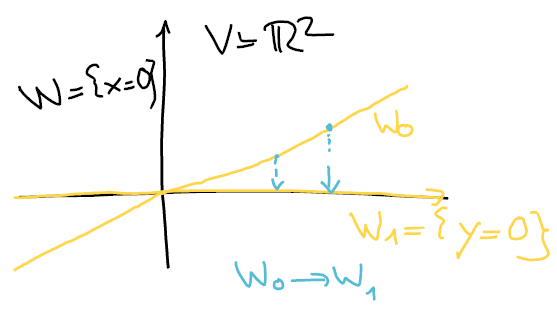
\includegraphics[width=0.5\linewidth]{figures/projektion_einschraenkung_auf_w_0}
        \label{fig:projektion_einschraenkung_auf_w_0}
    \end{figure}
    \begin{lemma}\label{projektion_isomorph}
        Sei \( V \) ein \( K \)-Vektorraum, \( W,W_0, W_1\subseteq V \) Untervektorräume mit \( V=W\oplus W_0=W\oplus W_1 \).

        Dann ist \( \evaluateat{P_W}{W_0}\maps W_0\to W_1 \) ein Isomorphismus (Notation wie oben).
    \end{lemma}
    \begin{proof}
        Es gilt \( \dim W_0=\dim W_1 \) und es genügt zu zeigen, dass \( \evaluateat{P_W}{W_0} \) injektiv ist.

        Sei \( \evaluateat{P_W}{w_0}=w_1 \) für \( w_0\in W_0 \), \( w_1\in W_1 \). Dann ist \( w_0=w+w_1 \) mit \( w\in W \), \( w_1\in W_1 \), also
        \begin{align*}
            w_1=\underrelate{\textcolor{LimeGreen}{\vertni}}{\textcolor{LimeGreen}{W_0}}{w_0}-\underrelate{\textcolor{LimeGreen}{\vertni}}{\textcolor{LimeGreen}{W}}{w}\in W_0\oplus W,
        \end{align*}
        und diese Zerlegung ist eindeutig.
        
    \end{proof}
    
\end{wiederholung*}
\subsection*{Parallelprojektionen für affine Räume}
Sei \( X \) ein affiner Raum (über einem Körper \( K \)), \( Y_1\subseteq X \) ein affiner Unterraum
\begin{beispiel*}
    \begin{figure}[H]
        \centering
        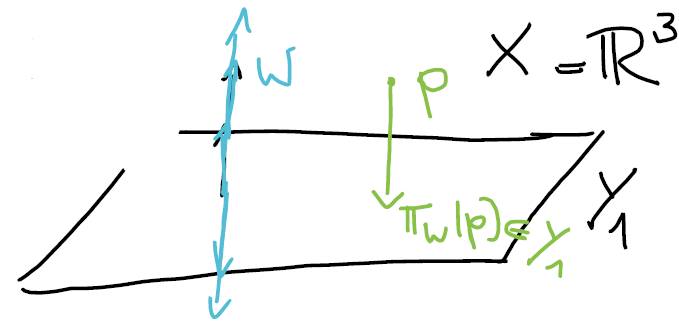
\includegraphics[width=0.5\linewidth]{figures/affine_parallelprojektion_r_3}
        \label{fig:affine_parallelprojektion_r_3}
    \end{figure}
    
\end{beispiel*}
Sei \( W\subseteq T(X) \) ein Untervektorraum mit \( T(X)=T(Y_1)\oplus W \).
\begin{ziel*}
    Definiere eine Projektionsabbildung
    \begin{align*}
        \pi_W\maps X\to Y_1
    \end{align*}
    \enquote{längs \( W \)}.
\end{ziel*}
Für \( p\in X \) definiere
\begin{align*}
    W(p)\definedas\Set{x\in X| \vv{px}\in W}
\end{align*}
\begin{lemma}
    Notation wie oben.
    Für \( p\in X \) gilt
    \begin{align*}
        \anzahl(Y_1\cap W(p))=1.
    \end{align*}
\end{lemma}
\begin{proof}
    Wir berechnen
    \begin{align*}
        \dim(Y_1\cap W(p)).
    \end{align*}
    Sei \( x=\dim X \), verwende \thref{verbindungsraum:dimension}~\ref{verbindungsraum:dimension:schnitt_leer}.
    Falls \( Y_1\cap W(p)=\emptyset \), dann
    \begin{align*}
        \dim(Y_1\vee W(p))\begin{aligned}[t] 
            &=\dim Y_1+\dim W(p)-\dim(\underbrace{T(Y_1)\cap W}_{\textcolor{LimeGreen}{=\zeroset}})+1\\
            &=\dim T(Y_1)+\dim W+1
        \end{aligned}
    \end{align*}
    \contra zu \( Y_1\vee W(p)\subseteq X \), also ist \( Y_1\cap W(p)\neq \zeroset \), und nach \thref{verbindungsraum:dimension}~\ref{verbindungsraum:dimension:schnitt_nicht_leer} gilt Folgendes:
    \begin{align*}
        \equalto{n}{\underbrace{\dim (Y_1\vee W(p))}}\begin{aligned}[t] 
            &=\dim Y_1+\dim W(p)-\dim(Y_1\cap W(p))\\
            &=n-\dim(Y_1\cap W(p))
        \end{aligned}
    \end{align*}
    und nach \thref{schnittraum:translationen}
    \begin{align*}
        \dim Y_1\vee W(p)\begin{aligned}[t] 
            &=\dim(T(Y_1)+W)\\
            &=n,
        \end{aligned}
    \end{align*}
    also \( \dim(Y_1\cap W(p))=0 \).
    
\end{proof}
Wir definieren die Projektion längs \( W \)
\begin{align*}
    \pi_W\maps \underrelate{\subseteq}{Y_0}{X}\to Y_1,\logicspace p\mapsto W(p)\cap Y_1.
\end{align*}
\begin{satz}
    Sei \( X \) ein affiner Raum, \( Y_1,Y_0\subseteq X \) affine Unterräume, \( W\subseteq T(X) \) ein Untervektorraum mit 
    \begin{align*}
        T(X)=W\oplus T(Y_0)=W\oplus T(Y_1).
    \end{align*}
    Dann ist \( \pi_W\maps X\to Y_1 \) eine surjektive affine Abbildung und \( \evaluateat{\pi_w}{Y_0}\maps Y_0\to Y_1 \) eine Affinität.
\end{satz}
\begin{proof}
    Seien \( p,q\in X \).
    \begin{figure}[H]
        \centering
        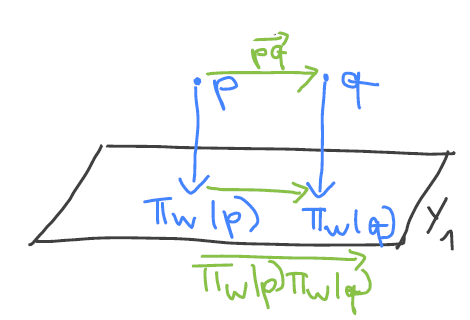
\includegraphics[width=0.5\linewidth]{figures/affine_projektion_ist_affin}
        \label{fig:affine_projektion_ist_affin}
    \end{figure}
    Dann gilt
    \begin{align*}
        \vv{pq}\begin{aligned}[t] 
            &=\vv{p\pi_W(p)}+\vv{\pi_W(p)\pi_W(q)}+\vv{\pi_W(q)q}+\vv{\pi_W(q)q}\\
            &=\underbrace{\vv{p\pi_W(p)}+\vv{\pi_W(q)q}}_{\textcolor{Cyan}{\in W}}+\underbrace{\vv{\pi_W(p)\pi_W(q)}}_{\textcolor{Cyan}{\in T(Y_1)}},
        \end{aligned}
    \end{align*}
    also \( \vv{\pi_W(p)\pi_W(q)}=P_W(\vv{pq}) \).

    \( P_W \) ist surjektiv, also ist \( \pi_W \) eine surjektive affine Abbildung.

    Der zweite Teil folgt aus \thref{projektion_isomorph}.
\end{proof}
% !TEX root = ./Vorlesungsmitschrift AGLA 2.tex  
\lecture{Di 28.04. 10:15}{}
\section{Affine Koordinaten}
Koordinaten in einem \( K \)-Vektorraum \( V \). Sei \( \dim V=n \) und \( v_1,\dotsc , v_n \) eine Basis von \( V \). Dann ist die Abbildung
\begin{align*}
    \phi\maps  \begin{aligned}[t]
        K^n&\to V\\
        (x_1,\dotsc,x_n)&\mapsto \sum\limits_{i=1}^{n}x_i v_i
    \end{aligned}
\end{align*}
ein Isomorphismus von \( K \)-Vektorräumen. Jeder Punkt \( \underrelate{\ni}{V}{v}=\sum_{i=1}^{n}x_i v_i \) ist eindeutig bestimmt durch seine \enquote{Koordinaten}
\begin{align*}
    \inf{\phi}(v)=(x_1,\dotsc,x_n)\in K^n.
\end{align*}
\begin{frage*}
    Sei \( X \) ein affiner Raum über einem Körper \( K \). Können wir auch hier die Lage eines Punkte \( p\in X \) durch Angabe von \enquote{Koordinaten} bezüglich einer \enquote{Basis} beschreibe?
    \begin{figure}[H]
        \centering
        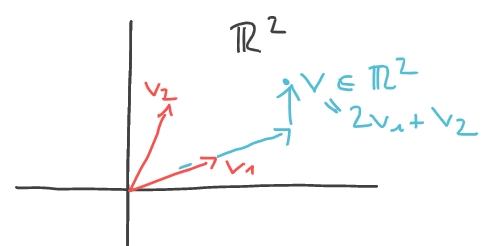
\includegraphics[width=0.5\linewidth]{figures/affine_koordinaten_r_2_hoffnung}
        \label{fig:affine_koordinaten_r_2_hoffnung}
    \end{figure}
    
\end{frage*}
\begin{bspidee*}
    \( X=\reals^2 \) als affiner Raum und Punkte \( p_1,p_2\in X \), sodass \( \vv{p_0p_1} \), \( \vv{p_0p_2} \) eine Basis ist für \( T(X) \). Dann können wir einen Punkt \( p\in X \) beschreiben durch
    \begin{align*}
        p \begin{aligned}[t]
            &=\tau_{\vv{p_0p}}(p_0)\\
            &=\tau_{\lambda\vv{p_0p_1}+\mu\vv{p_0p_2}}(p_0),
        \end{aligned}
    \end{align*}
    falls \( \vv{p_0p}=\lambda\vv{p_0p_1}+\mu\vv{p_0p_2} \) mit \( \lambda,\mu\in \reals \).

    \begin{figure}[H]
        \centering
        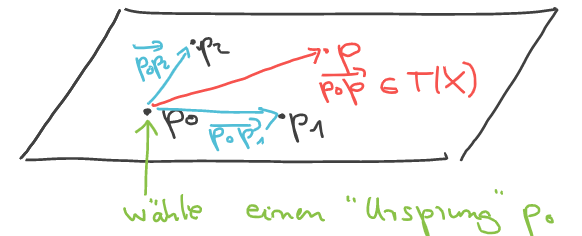
\includegraphics[width=0.5\linewidth]{figures/ursprungswahl}
        \label{fig:ursprungswahl}
    \end{figure}
    
    Wir erhalten eine Abbildung 
    \begin{align*}
        \phi\maps \begin{aligned}[t]
            \reals^2&\to X\\
            (\lambda,\mu)&\mapsto \tau_{\lambda\vv{p_0 p_1}+\mu\vv{p_0 p_2}}(p_0),
        \end{aligned}
    \end{align*}
    die eine Affinität ist.
\end{bspidee*}
Wir formalisieren diese Konzepte für allgemeine affine Räume.
\begin{definition*}
    Sei \( X \) ein affiner Raum und \( p_0,\dotsc, p_n\in X \). Wir nennen \( (p_0,\dotsc,p_n) \) \emph{affin unabhängig} \bzw eine \emph{affine Basis}, wenn die Vektoren \( (\vv{p_0p_1},\dotsc, \vv{p_0p_n}) \) in \( T(x) \) \emph{linear unabhängig sind} \bzw \emph{eine Basis bilden}.
\end{definition*}
\begin{beispiele*}
    \begin{enumerate}
        \item In \( X=\reals^n \) ist \( (0,e_1,\dotsc, e_n) \) eine affine Basis.
        \item \( X=\reals^n \) als affiner Raum, \( v_1,\dotsc, v_k\in \reals^n \) linear unabhängig, \( v_0=0 \). Dann ist das Tupel \( (v_0,v_1,\dotsc,v_k) \) affin unabhängig.
        \begin{frage*}
            Kann man hier \( v_0\in \reals^n \) beliebig nehmen?
        \end{frage*}
        \item \( X=\reals^2 \) als affiner Raum. Dann gilt, dass für \( v,w\in \reals^2 \) das Tupel \( (v,w) \) affin unabhängig ist \gdw \( v\neq w \).
        \item \( X \) affiner Raum, \( p_0\in X \), \( (t_1,\dotsc,t_n) \) Basis von \( T(X) \). Dann ist
        \begin{align*}
            (p_0,\tau_{t_1}(p_0),\dotsc, \tau_{t_n}(p_0))
        \end{align*}
        eine affine Basis von \( X \).
    \end{enumerate}
    
\end{beispiele*}
\begin{lemma}
    Sei \( X \) ein affiner Raum, \( p_0,\dotsc, p_n\in X \) und \( (p_0,\dotsc, p_n) \) affin unabhängig. Sei \( \sigma\in S_{n+1} \) eine Permutation von \( \Set{0,\dotsc,n} \). Dann ist
    \begin{align*}
        (p_{\sigma(0)},p_{\sigma(1)},\dotsc,p_{\sigma(n)})
    \end{align*}
    affin unabhängig.
\end{lemma}
\begin{proof}
    Wir wollen zeigen, dass unter den Annahmen des Lemmas, die Vektoren
    \begin{align*}
        \vv{p_{\sigma(0)}p_{\sigma(1)}},\dotsc,\vv{p_{\sigma(0)p_{\sigma(n)}}}\in T(X)
    \end{align*}
    linear unabhängig sind.

    Sei \( \sigma(0)=i\in \Set{0,\dotsc,n} \).

    Dann müssen wir also zeigen, dass die Vektoren
    \begin{align*}
        \vv{p_i p_0},\vv{p_i p_1},\dotsc, \vv{p_i p_{i-1}},\vv{p_i p_{i+1}},\dotsc,\vv{p_i p_n}
    \end{align*}
    linear unabhängig sind.

    Seien \( \lambda_0,\dotsc, \lambda_{i-1},\lambda_{i+1},\dotsc,\lambda_n\in K \) mit
    \begin{align*}
        \lambda_0 \vv{p_i p_0}+\lambda_1\vv{p_i p_1}+\dotsb+\lambda_{i-1}\vv{p_i p_{i-1}}+\lambda_{i+1}\vv{p_i p_{i+1}}+\dotsb+\lambda_n\vv{p_i p_n}=0.
    \end{align*}
    Schreibe
    \begin{align*}
        \vv{p_i p_j}=\vv{p_i p_0}+\vv{p_0 p_j}=\textcolor{Goldenrod}{\vv{p_0 p_j}}-\textcolor{LimeGreen}{\vv{p_0 p_i}}.
    \end{align*}
    Wir erhalten
    \begin{align*}
        \begin{aligned}[t]
            \textcolor{Goldenrod}{\lambda_1\vv{p_0 p_1}+\dotsb+\lambda_{i-1} \vv{p_0 p_{i-1}}+\lambda_{i+1} \vv{p_0 p_{i+1}}+\dotsb+\lambda_n \vv{p_0 p_n}}\\
            -\textcolor{LimeGreen}{(\lambda_0+\dotsb+\lambda_{i-1}+\lambda_{i+1}+\dotsb+\lambda_n)\vv{p_0 p_i}}=0
        \end{aligned}
    \end{align*}
    Aus der linearen Unabhängigkeit von \( \vv{p_0 p_1},\dotsc, \vv{p_0 p_n} \) folgt
    \begin{align*}
        \lambda_1=\dotsb=\lambda_{i-1}=\lambda_{i+1}=\lambda_n=0
    \end{align*}
    und
    \begin{align*}
            \explain{\lambda_0=0}+\underbrace{\lambda_1+\dotsb+\lambda_{i-1}+\lambda_{i+1}+\dotsb+\lambda_n}_{=0}=0
    \end{align*}
\end{proof}
\subsection*{Affine Basen und affine Abbildungen}
Aus der AGLA \Romannum{1}:\\
Seien \( V,W \) \( K \)-Vektorräume, \( v_1,\dotsc, v_n \in V \) eine Basis von \( V \) und \( w_1,\dotsc, w_n \in W\). Dann gibt es genau eine \( K \)-lineare Abbildung \( \phi\maps V\to W \) mit
\begin{align*}
    \phi(v_i)=w_i,\quad 1\leq i \leq n.
\end{align*}
\begin{figure}[H]
    \centering
    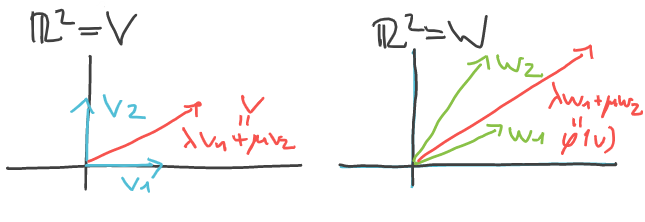
\includegraphics[width=0.7\linewidth]{figures/bilder_der_basen_bestimmt_abbildung_r_2}
    \label{fig:bilder_der_basen_bestimmt_abbildung_r_2}
\end{figure}
\begin{frage*}
    Inwiefern sind affine Abbildungen zwischen affinen Räumen durch die Bilder einer affinen Basis bestimmt?
\end{frage*}
\begin{satz}\label{bilder_der_basen_bestimmen_affine_abbildung}
    Seien \( X,Y \) affine Räume, \( (p_0,\dotsc,p_n) \) eine affine Basis von \( X \) und \( q_0,\dotsc, q_n\in Y \). Dann gibt es genau eine affine Abbildung \( f\maps X\to Y \) mit
    \begin{align*}
        f(p_i)=q_i,\quad 0\leq i\leq n.
    \end{align*}
    Die Abbildung \( f \) ist \emph{injektiv} \bzw \emph{eine Affinität} \gdw das Tupel \( (q_0,\dotsc, q_n) \) \emph{affin unabhängig} \bzw \emph{eine affine Basis} von \( Y \) ist.
\end{satz}
\begin{proof}
    Eine affine Abbildung \( f\maps X\to Y \) ist gegeben durch \( f(p_0) \) für ein \( p_0\in X \) und eine lineare Abbildung
    \begin{align*}
        F\maps \begin{aligned}[t]
            T(X)&\to T(Y)\\
            \vv{pq}&\mapsto \vv{f(p)f(q)}.
        \end{aligned}
    \end{align*}
    Wir definieren \( F \) durch
    \begin{align*}
        F(\vv{p_0 p_i})=\vv{q_0 q_i}\quad 1\leq i \leq n. \tag{*}\label{bilder_der_basen_bestimmt_affine_abbildung:beweis:k_lineare_abbildung}
    \end{align*}
    \( \vv{p_0 p_1}, \dotsc, \vv{p_0 p_n} \) ist eine Basis von \( T(X) \), also gibt es genau ein lineare Abbildung
    \begin{align*}
        F\maps T(X)\to T(Y)
    \end{align*}
    mit \eqref{bilder_der_basen_bestimmt_affine_abbildung:beweis:k_lineare_abbildung}. Es gilt dann
    \begin{align*}
        f(p_i)\begin{aligned}[t]
            &=\tau_{\vv{f(p_0) f(p_i)}} f(p_0)\\
            &=\tau_{F(\vv{p_0 p_i})} f(p_0)\\
            &=\tau_{\vv{q_0 q_i}} q_0 =q_i \quad 1\leq i \leq n.
        \end{aligned}
    \end{align*}
    \( f \) ist injektiv \gdw \( F \) injektiv ist. \( F \) ist injektiv \gdw \( \vv{q_0 q_1}, \dotsc, \vv{q_0 q_n} \) linear unabhängig sind.

    \tto \( f \) ist eine Affinität \gdw \( F \) bijektiv ist. \( F \) ist bijektiv \gdw \( \vv{q_0 q_1}, \dotsc, \vv{q_0 q_n} \) eine Basis von \( T(Y) \) ist.

\end{proof}
\subsection*{Affine Koordinatensysteme}
Sei \( X \) ein affiner Raum über einem Körper \( K \), \( (p_0,p_1,\dotsc, p_n) \) eine affine Basis von \( X \).

Nach \thref{bilder_der_basen_bestimmen_affine_abbildung} gibt es genau eine Affinität
\begin{align*}
    \phi\maps K^n\to X
\end{align*}
mit \( \phi(0)=p_0, \phi(e_1)=p_1,\dotsc, \phi(e_n)=p_n \) und zugehörige lineare Abbildung \( \Phi\maps K^n \to T(X) \).

Einen Punkt \( p\in X \) können wir dann beschreiben durch
\begin{align*}
    p=\tau_{\vv{p_0 p}}(p_0).
\end{align*}
Sei \( \vv{p_0 p}=\lambda_1 \vv{p_0 p_1}+\dotsb +\lambda_n \vv{p_0 p_n} \) mit \( \lambda_i\in K \), \( 1\leq i \leq n \).

Dann ist
\begin{align*}
    p \begin{aligned}[t]
        &=\tau_{\lambda_1\vv{p_0 p_1}+\dotsb +\lambda_n\vv{p_0 p_n}}(p_0)\\
        &=\tau_{\lambda_1 \Phi(e_1)+\dotsb+\lambda_n \Phi(e_n)}(p_0)\\
        &=\tau_{\Phi(\lambda_1 e_1+\dotsb+\lambda_n e_n)}(p_0),
    \end{aligned}
\end{align*}
oder \( p=\phi((\lambda_1,\dotsc,\lambda_n)) \).

\begin{definition*}
    Sei \( X \) ein affiner Raum über einem Körper \( K \). Wir nennen eine Affinität \( \phi\maps K^n\to X \) ein affines Koordinatensystem in \( X \). Seu \( p_0=\phi(0),p_1=\phi(e_1),\dotsc, p_n=\phi(e_n) \). Dann ist \( (p_0,\dotsc,p_n) \) eine affine Basis von \( X \).

    Für \( p\in X \) nennen wir
    \begin{align*}
        \inv{\phi}(p)=(x_1,\dotsc,x_n)\in K^n
    \end{align*}
    den Koordinatenvektor von \( p \) bezüglich der affinen Basis \( (p_0,\dotsc,p_n) \) und \( (x_1,\dotsc, x_n) \) die Koordinaten von \( p \) bezüglich \( (p_0,\dotsc, p_n) \).
    \begin{figure}[H]
        \centering
        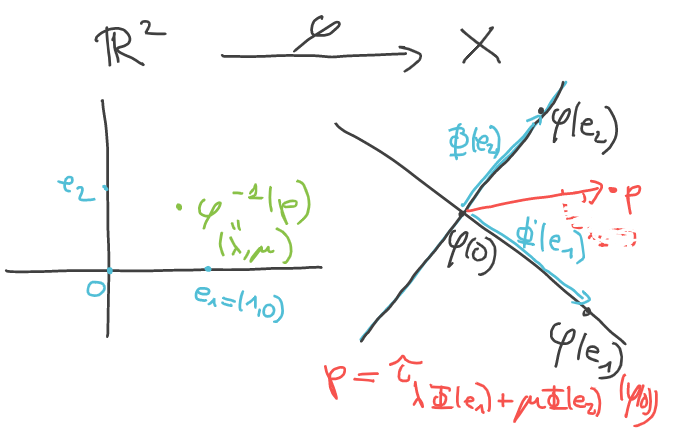
\includegraphics[width=0.7\linewidth]{figures/affine_koordinatenabbildung_r_2}
        \label{fig:affine_koordinatenabbildung_r_2}
    \end{figure}
\end{definition*}
\section{Das Teilverhältnis}
\begin{idee*}
    Seien 3 Punkte \( p_0,p_1,p \) auf einer Gerade \( l \) (\zb im \( \reals^3 \)) gegeben, \( p_0\neq p_1 \).
    \begin{figure}[H]
        \centering
        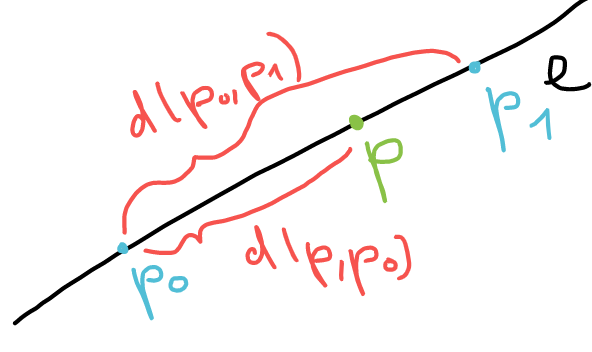
\includegraphics[width=0.5\linewidth]{figures/gerade_teilverhaeltnis}
        \caption*{}
        \label{fig:gerade_teilverhaeltnis}
    \end{figure}
    Sei \( \lambda=\frac{d(p,p_0)}{d(p_1,p_0)} \), mit \( d \) dem euklidischen Abstand, dann können wir die Lage von \( p \) auf \( l \) durch \( \lambda \) (und der Information, ob \( p \) \enquote{rechts oder links} von \( p \) liegt) bestimmen.
\end{idee*}
\begin{definition*}
    Sei \( X \) ein affiner Raum über \( K \), \( Y\subseteq X \) eine affine Gerade, \( p_0,p_1,p\in Y \) und \( p_0\neq p_1 \). Dann nennen wir das eindeutig bestimmte Element \( \lambda\in K \) mit \( \vv{p_0 p}=\lambda \vv{p_0 p_1} \) das Teilverhältnis von \( p_0,p_1,p \). Schreibe \( \lambda=\teilverhaeltnis(p_0,p_1,p) \). In \( \characteristic(K)\neq 2 \) nennen wir \( p \) Mittelpunkt von \( p_0,p_2 \) wenn \( \teilverhaeltnis(p_0,p_1,p)=\frac{1}{2} \).
\end{definition*}
\begin{bemerkungen*}
    \begin{enumerate}
        \item Es gilt \( T(Y)=K\vv{p_0p_1} \). Damit ist \( \lambda \) wohldefiniert und existiert.
        \item \( p_0,p_1 \) ist eine affine Basis von \( Y \). Damit existiert ein Koordinatensystem
        \begin{align*}
            \phi\maps K\to Y,\logicspace \begin{aligned}[t]
                \phi(0)&=p_0\\
                \phi(1)&=p_1
            \end{aligned}
        \end{align*}
        und es gilt \( \teilverhaeltnis(p_0,p_1,p)=\inv{\phi(p)} \).
    \end{enumerate}
    
\end{bemerkungen*}
\begin{frage*}
    Wie verhält sich das Teilverhältnis unter affinen Abbildungen?
    \begin{figure}[H]
        \centering
        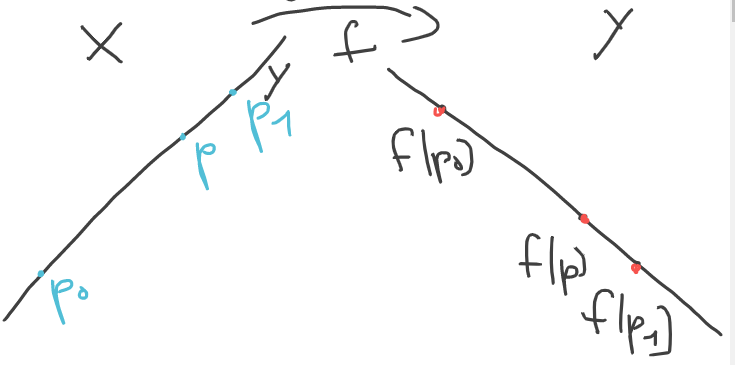
\includegraphics[width=0.7\linewidth]{figures/affine_abbildungen_wirkung_auf_teilverhaeltnis}
        \label{fig:affine_abbildungen_wirkung_auf_teilverhaeltnis}
    \end{figure}
    
\end{frage*}

\begin{lemma}\label{teilverhaeltnis_invariant_unter_affinen_abbildungen}
    Seien \( X,Y \) affine Räume und \( f\maps X\to Y \) eine affine Abbildung, seien \( p_0,p1,p \) Punkte in \( X \), die auf einer Geraden liegen und \( f(p_0)\neq f(p_1) \). Dann gilt
    \begin{align*}
        \teilverhaeltnis(f(p_0),f(p_1),f(p))=\teilverhaeltnis(p_0,p_1,p).
    \end{align*}
\end{lemma}
\begin{proof}
    Sei \( \lambda=\teilverhaeltnis(p_0,p_1,p) \), also \( \vv{p_0 p}=\lambda\vv{p_0 p_1} \). Si \( F\maps T(X)\to T(Y) \) die zu \( f \) gehörige lineare Abbildung. Wir berechnen
    \begin{align*}
        \vv{f(p_0) f(p)}\begin{aligned}[t]
            &=F(\vv{p_0 p})\\
            &=F(\lambda{p_0 p_1})\\
            &=\lambda F({p_0 p_1})\\
            &=\lambda \vv{f(p_0) f(p_1)}
        \end{aligned}
    \end{align*}
    
\end{proof}
\begin{anwendung*}[Strahlensatz]
    Sei \( X \) ein affiner Raum über \( K \), \( p_0,p_1,p_2\in X \) affin unabhängig. Sei
    \begin{align*}
        q_1&\in p_0\vee p_1,\logicspace q_1\neq p_0\\
        q_2&\in p_0\vee p_2,\logicspace q_2\neq p_0.
    \end{align*}
    Wir nehmen an, dass \( p_1\vee p_2 \) und \( q_1\vee q_2 \) parallel sind in dem Sinn, dass
    \begin{align*}
        T(p_1\vee p_2)=T(q_1\vee q_2)\text{ in }T(X).
    \end{align*}
    Dann gilt
    \begin{align*}
        \teilverhaeltnis(p_0,p_1,q_1)=\teilverhaeltnis(p_0,p_2,q_2).
    \end{align*}
    \begin{figure}[H]
        \centering
        \includegraphics[width=0.5\linewidth]{figures/Strahlensatz}
        \label{fig:Strahlensatz}
    \end{figure}
\end{anwendung*}
\begin{proof}
    Sei \( Y \) diedurch \( p_0,p_1,p_2 \) aufgespannte Ebene. Dann gibt es ein affines Koordinatensystem \( \phi\maps K^2 \to Y \) mit \( \phi(0)=p_0, \phi(e_1)=p_1, \phi(e_2)=p_2 \).
    \begin{figure}[H]
        \centering
        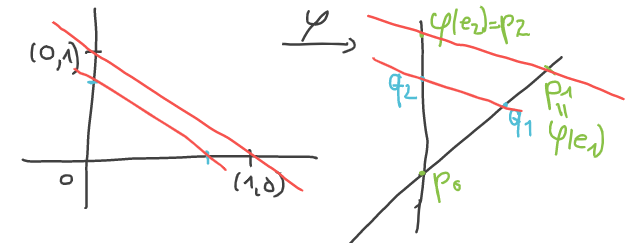
\includegraphics[width=0.5\linewidth]{figures/strahlensatz_koordinatensystem}
        \label{fig:strahlensatz_koordinatensystem}
    \end{figure}
    Sei
    \begin{align*}
        (\lambda,0)&=\inv{\phi}(q_1)\\
        (0,\mu)&=\inv{\phi}(q_2).
    \end{align*}    
    \begin{behauptung*}
        \( l_1=\inv{\phi}(q_1)\vee \inv{\phi}(q_2) \) und \( l_2=\inv{\phi}(p_1)\vee \inv{\phi}(p_2) \) sind parallel.
    \end{behauptung*}
    \minisec{Denn:}
    \begin{align*}
        T(l_1)&=K\vv{\inv{\phi}(q_1) \inv{\phi}(q_2)}\\
        T(l_2)&=K\vv{\inv{\phi}(p_1) \inv{\phi}(p_2)}.
    \end{align*}
    Es ist \( K\vv{p_1 p_2}=K\vv{q_1 q_2} \) und daher
    \begin{align*}
        \equalto{K\vv{\inv{\phi}(q_1) \inv{\phi}(q_2)}}{K \inv{\Phi}(\vv{p_1 p_2})}=\equalto{K\vv{\inv{\phi}(p_1) \inv{\phi}(p_2)}}{K\inv{\Phi}(\vv{q_1 q_2}}).
    \end{align*}
    Aus der Parallelität von \( l_1,l_2 \) folgt \( \lambda=\mu \).

    Also
    \begin{align*}
        &\rphantom{=}\teilverhaeltnis(\inv{\phi}(p_0),\inv{\phi}(p_1),\inv{\phi}(q_1))=\lambda\\
        &=\mu=\teilverhaeltnis(\inv{\phi}(p_0),\inv{\phi}(p_2),\inv{\phi}(q_2))
    \end{align*}
    und der Strahlensatz folgt aus \thref{teilverhaeltnis_invariant_unter_affinen_abbildungen}.
\end{proof}


% !TEX root = ./Vorlesungsmitschrift AGLA 2.tex  
\lecture{Di 05.05. 10:15}{}
\begin{lemma}\label{teilverhaeltnis_invariant_unter_affinen_abbildungen}
    Seien \( X,Y \) affine Räume und \( f\maps X\to Y \) eine affine Abbildung, seien \( p_0,p1,p \) Punkte in \( X \), die auf einer Geraden liegen und \( f(p_0)\neq f(p_1) \). Dann gilt
    \begin{align*}
        \teilverhaeltnis{f(p_0)}{f(p_1)}{f(p)}=\teilverhaeltnis{p_0}{p_1}{p}.
    \end{align*}
\end{lemma}
\begin{proof}
    Sei \( \lambda=\teilverhaeltnis{p_0}{p_1}{p} \), also \( \vv{p_0 p}=\lambda\vv{p_0 p_1} \). Sei \( F\maps T(X)\to T(Y) \) die zu \( f \) gehörige lineare Abbildung. Wir berechnen
    \begin{align*}
        \vv{f(p_0) f(p)}\begin{aligned}[t]
            &=F(\vv{p_0 p})\\
            &=F(\lambda{p_0 p_1})\\
            &=\lambda F({p_0 p_1})\\
            &=\lambda \vv{f(p_0) f(p_1)}
        \end{aligned}
    \end{align*}
    
\end{proof}
\begin{anwendung*}[Strahlensatz]
    Sei \( X \) ein affiner Raum über \( K \), \( p_0,p_1,p_2\in X \) affin unabhängig. Sei
    \begin{align*}
        q_1&\in p_0\vee p_1,\logicspace q_1\neq p_0\\
        q_2&\in p_0\vee p_2,\logicspace q_2\neq p_0.
    \end{align*}
    Wir nehmen an, dass \( p_1\vee p_2 \) und \( q_1\vee q_2 \) parallel sind in dem Sinn, dass
    \begin{align*}
        T(p_1\vee p_2)=T(q_1\vee q_2)\text{ in }T(X).
    \end{align*}
    Dann gilt
    \begin{align*}
        \teilverhaeltnis{p_0}{p_1}{q_1}=\teilverhaeltnis{p_0}{p_2}{q_2}.
    \end{align*}
    \begin{figure}[H]
        \centering
        \includegraphics[width=0.5\linewidth]{figures/Strahlensatz}
        \label{fig:Strahlensatz}
    \end{figure}
\end{anwendung*}
\begin{proof}
    Sei \( Y \) diedurch \( p_0,p_1,p_2 \) aufgespannte Ebene. Dann gibt es ein affines Koordinatensystem \( \phi\maps K^2 \to Y \) mit \( \phi(0)=p_0, \phi(e_1)=p_1, \phi(e_2)=p_2 \).
    \begin{figure}[H]
        \centering
        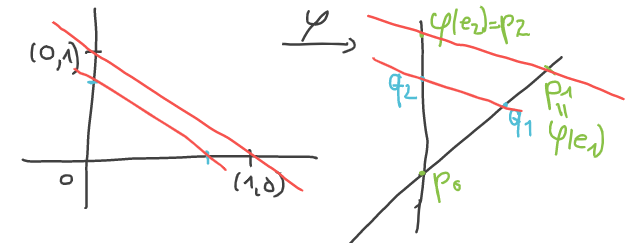
\includegraphics[width=0.5\linewidth]{figures/strahlensatz_koordinatensystem}
        \label{fig:strahlensatz_koordinatensystem}
    \end{figure}
    Sei
    \begin{align*}
        (\lambda,0)&=\inv{\phi}(q_1)\\
        (0,\mu)&=\inv{\phi}(q_2).
    \end{align*}    
    \begin{behauptung*}
        \( l_1=\inv{\phi}(q_1)\vee \inv{\phi}(q_2) \) und \( l_2=\inv{\phi}(p_1)\vee \inv{\phi}(p_2) \) sind parallel.
    \end{behauptung*}
    \minisec{Denn:}
    \begin{align*}
        T(l_1)&=K\vv{\inv{\phi}(q_1) \inv{\phi}(q_2)}\\
        T(l_2)&=K\vv{\inv{\phi}(p_1) \inv{\phi}(p_2)}.
    \end{align*}
    Es ist \( K\vv{p_1 p_2}=K\vv{q_1 q_2} \) und daher
    \begin{align*}
        \equalto{K\vv{\inv{\phi}(q_1) \inv{\phi}(q_2)}}{K \inv{\Phi}(\vv{p_1 p_2})}=\equalto{K\vv{\inv{\phi}(p_1) \inv{\phi}(p_2)}}{K\inv{\Phi}(\vv{q_1 q_2}}).
    \end{align*}
    Aus der Parallelität von \( l_1,l_2 \) folgt \( \lambda=\mu \).

    Also
    \begin{align*}
        &\rphantom{=}\teilverhaeltnis{\inv{\phi}(p_0)}{\inv{\phi}(p_1)}{\inv{\phi}(q_1)}=\lambda\\
        &=\mu=\teilverhaeltnis{\inv{\phi}(p_0)}{\inv{\phi}(p_2)}{\inv{\phi}(q_2)}
    \end{align*}
    und der Strahlensatz folgt aus \thref{teilverhaeltnis_invariant_unter_affinen_abbildungen}.
\end{proof}
\file{Affinkombinationen}
\section{Affinkombinationen}
\begin{beispiel*}
    Seien \( p_0,p_1\in \reals^2 \), \( p_0\neq p_1 \). Ziel: Beschreibe den affinen Unterraum \( p_0\vee p_1 \) als Teilmenge des \( \reals^2 \). Sei \( p\in p_0\vee p_1 \). Dann \( \exists \lambda\in \reals \) mit \( \vv{p_0 p}=\lambda \vv{p_0 p_1} \) und als Vektoren im \( \reals^2 \) gilt \( p=p_0+\lambda(p_1-p_0) \). Es gilt
    \begin{align*}
        p_0 \vee p_1=\Set{(1-\lambda)p_0+\lambda p_1,\logicspace \lambda\in \reals}.
    \end{align*}
    \begin{figure}[H]
        \centering
        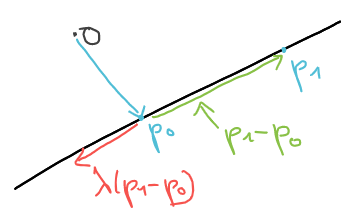
\includegraphics[width=0.5\linewidth]{figures/affine_verbindungsgerade}
        \label{fig:affine_verbindungsgerade}
    \end{figure}
    
\end{beispiel*}
\begin{frage*}
    Verallgemeinerung zu höherdimensionalen Räumen?
\end{frage*}
\begin{definition*}
    Seien \( p_0,\dotsc,p_k\in  K^n \). Wir nennen eine Linearkombination
    \begin{align*}
        \lambda_0 p_0+\lambda_1 p_1+\dotsb+\lambda_m p_m
    \end{align*}
    mit \( \lambda_i\in K \), \( 0\leq i\leq m \) eine Affinkombination oder affin falls gilt \( \lambda_0+\lambda_1+\dotsb+\lambda_m=1 \).
\end{definition*}
\begin{satz}
    Seien \( p_0,\dotsb,p_m\in K^n \). Dann gilt
    \begin{align*}
        p_0\vee \dotsb \vee p_m =\Set{\sum_{i=0}^{m}\lambda_i p_i\in K^n \logicspace \lambda_0,\dotsc,\lambda_m\in K, \sum_{i=0}^{m}\lambda_i=1}.
    \end{align*}
\end{satz}
\begin{proof}
    Sei \( Y=p_0 \vee\dotsb\vee p_m\in K^n \). Es gilt
    \begin{align*}
        T(Y)\begin{aligned}[t]
            &=\underbrace{T(p_m)}_{=0}+T(p_0\vee \dotsb \vee p_{m-1})+\underbrace{K\vv{p_0 p_m}}_{\mathclap{=T(p_0\vee p_m)}}\\
            &=K\vv{p_0 p_m}+T(p_0\vee \dotsb\vee p_{m-1})\\
            &=K\vv{p_0 p_m}+\dotsb +K\vv{p_0 p_1}\\
            &\vdots\\
            &=K\vv{p_0 p_m}+\dotsb + K\vv{p_0 p_1}\\
            &=\span(\vv{p_0 p_1}, \dotsc, \vv{p_0 p_m}).
        \end{aligned}
    \end{align*}
    Sei \( p\in K^n \). Dann ist \( p\in Y \) genau dann, wenn \texists \( \lambda_1,\dotsc,\lambda_m\in K \) mit
    \begin{align*}
        \vv{p_0 p}=\lambda_1 \vv{p_0 p_1}+\dotsb+\lambda_m\vv{p_0 p_m}.
    \end{align*}
    Im \( K^n \) gilt dann also
    \begin{align*}
        p-p_0=\lambda_1(p_1-p_0)+\dotsb + \lambda_m(p_m-p_0)
    \end{align*}
    oder 
    \begin{align*}
        p=\lambda_0 p_0+\lambda_1 p_1+\dotsb+\lambda_m p_m
    \end{align*}
    mit \( \lambda_0=1-\lambda_1-\dotsb-\lambda_m \), \dh \( \sum\limits_{i=0}^{m}\lambda_i=1 \).
\end{proof}
\file{Affine Abbildungen durch Matrizen, Fixpunkte}
\section{Affine Abbildungen und Matrizen, Fixpunkte}
\begin{motivation*}
    Seien \( V,W \) \( K \)-Vektorräume, \( F\maps V\to W \) eine lineare Abbildung. Wenn wir für \( V \) und \( W \) Basen wählen, dann können wir die Abbildung \( F \) eindeutig durch eine Matrix beschreiben.
\end{motivation*}
\begin{frage*}
    Inwiefern können wir affin Abbildung zwischen affinen Räumen durch Matrizen beschreiben?
\end{frage*}
Wahl von Basen in Vektorräumen \( \leftrightarrow \) Wahl von Koordinaten in affinen Räumen. 

Seien \( X,Y \) affine Räume über \( K \), \( f\maps X\to Y \) eine affine Abbildung. Wähle affine Koordinatensysteme \( \phi\maps K^n\to X  \) und \( \psi\maps K^m\to Y \).

Wir haben das folgende kommutative Diagramm
\begin{equation*}
    \begin{tikzcd}
        K^n\arrow{r}{\phi}\arrow{d}[name=g]{g} &X\arrow{d}[name=f]{f}\\
        K^m\arrow{r}{\psi}&Y
        \arrow[to path={(f) node[midway,scale=1] {\rotatebox{90}{\(\circlearrowright\)}} (g)}]{} 
    \end{tikzcd}    
\end{equation*}
mit \( g=\inv{\psi}\circ f\circ \phi \) affin. \( g \) ist affin, also besteht eine affine Abbildung \( G\maps K^n\to K^m \) mit
\begin{align*}
    g(x)-g(0)=G(x)\quad \forall x\in K^n.
\end{align*}
\( G \) ist linear, also können wir \( G \) durch eine Matrix \( A \) ausdrücken.
\begin{align*}
    g(x)=Ax+b\quad \forall x\in K^n.
\end{align*}
mit \( b=g(0) \).
\begin{frage*}
    Wie können wir \( A \) berechnen gegeben eine affine Basis \( (p_0,\dotsc,p_n) \) von \( K^n \) und \( g(p_i) \), \( 0\leq i \leq n \)?
\end{frage*}
\begin{figure}[H]
    \centering
    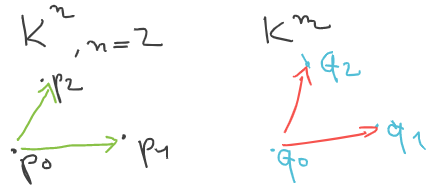
\includegraphics[width=0.5\linewidth]{figures/affine_basen_abbildung_wunsch}
    \label{fig:affine_basen_abbildung_wunsch}
\end{figure}
Wir betrachten die Matrizen \( B\in \matrices{m}{n}{K} \) bestehend aus den Spaltenvektoren \( \vv{q_0 q_1},\dotsc, \vv{q_0 q_n} \) und \( S\in \matrices{n}{n}{K} \) bestehend aus den Spaltenvektoren \( \vv{p_0 p_1}, \dotsc, \vv{p_0 p_n} \). Dann gilt \( A=B\cdot \inv{S}  \) und \( g(x)-g(p_0)=A(x-p_0) \), also \( g(x)=Ax+b \) mit \( b=g(p_0)-Ap_0 \).
\begin{bemerkung*}
    Wählen wir für \( p_0,\dotsc,pm \) die affine Basis \( 0,e_1,\dotsc, e_n \), dann \( S=\Id_{n\times n} \) und \( A=B \).
\end{bemerkung*}
\subsection*{Fixpunkte}
\begin{beispiel}
    Betrachte die affine Abbildung \( f\maps K\to K \), \( K \) ein Körper, in der Matrizendarstellung gegeben durch \( f(x)=2x+1\isittrue{=}x \).
    \begin{figure}[H]
        \centering
        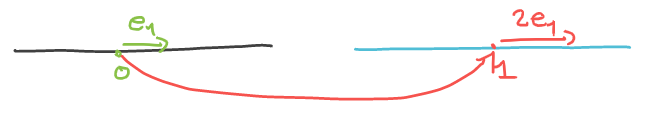
\includegraphics[width=0.5\linewidth]{figures/affiner_fixpunkt_1_d}
        \label{fig:affiner_fixpunkt_1_d}
    \end{figure}
    Dann gibt es genau ein \( x\in K \) mit \( f(x)=x \), nämlich \( x=-1 \).
\end{beispiel}
\begin{definition*}
    Sei \( X \) ein affiner Raum \( f\maps X\to X \) eine affine Abbildung. Wir nennen
    \begin{align*}
        \fixpunkte{f}\definedas \Set{x\in X|f(x)=x}
    \end{align*}
    die Menge der Fixpunkte von \( f \).
\end{definition*}
\begin{frage*}
    Welche Struktur hat \( \fixpunkte{f} \).
\end{frage*}
\begin{beispiel}
    \( X \) affiner Raum.
    \begin{align*}
        \Id\maps \begin{aligned}[t]
            X&\to X\\
            x&\mapsto x
        \end{aligned}
    \end{align*}
    dann \( \fixpunkte{\Id}=X \).
\end{beispiel}
\begin{beispiel}
    \( f\maps K^n\to K^n \), \( x\mapsto \underrelate{\isittrue{=}}{x}{\underbrace{x+p_0}} \) mit \( p_0\in K^n\setminus \zeroset \), dann \( \fixpunkte{f}=\emptyset \).
\end{beispiel}
\begin{beispiel}
    \begin{frage*}
        Was sind die Fixpunkte einer Projektion?
    \end{frage*}
    
\end{beispiel}
\begin{lemma}\label{affine_fixpunkte_sind_affiner_unterraum}
    \( \fixpunkte{f}\subseteq X \) ist ein affiner Unterraum.
\end{lemma}
\begin{proof}
    Falls \( \fixpunkte{f}=\emptyset \) dann \checkmark. Sei also \( \fixpunkte{f}\neq \emptyset \) und \( p\in \fixpunkte{f} \), \( F \) die zu \( f \) gehörig lineare Abbildung.

    Für \( x\in \fixpunkte{f} \) gilt
    \begin{align*}
        \vv{px}=\vv{f(p) f(x)}=F(\vv{px}).
    \end{align*}
    Umgekehrt folgt aus
    \begin{align*}
        \vv{px}=F(\vv{px})=\vv{p f(x)},
    \end{align*}
    dass \( x=f(x) \), also \( x\in \fixpunkte{f} \).

    Damit gilt
    \begin{align*}
        \Set{\vv{px}\in T(X)|x\in \fixpunkte{f}}=\Set{\vv{px}\in T(X)|\vv{px}=F(\vv{px})}
    \end{align*}
    und wir erkennen diese Menge als \( K \)-Untervektorraum von \( X \).
\end{proof}
\begin{frage*}
    Bestimmung von \( \fixpunkte{f} \) für eine beliebige affine Abbildung \( f\maps X\to X \)?
\end{frage*}
Nach Wahl eines Koordinatensystems können wir auf den Fall \( X=K^n \) reduzieren und annehmen, dass \( f \) in Matrizendarstellung gegeben ist.

Sei also
\begin{align*}
    f\maps \begin{aligned}[t]
        K^n&\to K^n\\
        x\mapsto &\underbrace{Ax+b}_{=x=\Id_n x}.
    \end{aligned}
\end{align*}
Dann gilt
\begin{align*}
    \fixpunkte{f}=\set{x\in K^n|(A-\explain{\text{Einheitsmatrix der Dimension \( n \):}\ \begin{pNiceMatrix}
        1 &  & 0 \\
         & \ddots &  \\
        0 &  & 1
    \end{pNiceMatrix}
    }{\Id_n})x=-b}
\end{align*}
Wir haben das Problem also reduziert auf das Lösen eines linearen Gleichungssystems.
\begin{bemerkung*}
    Daraus kann man auch \thref{affine_fixpunkte_sind_affiner_unterraum} ableiten.
\end{bemerkung*}
\begin{beispiel}\label{dilatation_beispiel}
    \begin{align*}
        f\maps \begin{aligned}[t]
            K^n&\to K^n\\
            x&\mapsto \lambda \Id_n x+b
        \end{aligned}     
    \end{align*}
    mit \( \lambda\in K \).

    Dann
    \begin{align*}
        \fixpunkte{f}=\Set{x\in K^n|(\lambda-1)x=-b}.
    \end{align*}
    Falls \( \lambda-1 \) invertierbar ist \( (\lambda\neq 1) \), gibt es genau einen Fixpunkt.
\end{beispiel}
\begin{definition*}
    Sei \( f\maps X\to X \) eine affine Abbildung mit zugehöriger linearer Abbildung \( F\maps T(X)\to T(X) \). Wir nennen \( f \) eine \emph{Dilatation} mit \emph{Faktor \( \lambda \)}, falls gilt
    \begin{align*}
        F=\lambda \cdot \Id_{T(X)}\quad \lambda\in K.
    \end{align*}
    Im Fall \( \lambda=1 \) nennen wir \( f \) eine Translation.
\end{definition*}
\begin{lemma}
    Sei \( f\maps X\to X \) eine Dilatation mit Faktor \( \lambda\neq 1 \). Dann gilt
    \begin{align*}
        \anzahl-{\fixpunkte{f}}=1.
    \end{align*}
\end{lemma}
\begin{proof}
    Nach Wahl eines Koordinatensystems reduzieren wir das Problem auf \thref{dilatation_beispiel}.    
\end{proof}
\file{Kollineationen}
\section{Kollineationen}
Sei \( f\maps X\to X \) eine affine Abbildung eines affinen Raumes \( X \), \zb eine Affinität. Seien \( p_1,p_2,p_3\subset X \) in einer Geraden \( \ell\subseteq X \) enthalten.
\begin{figure}[H]
    \centering
    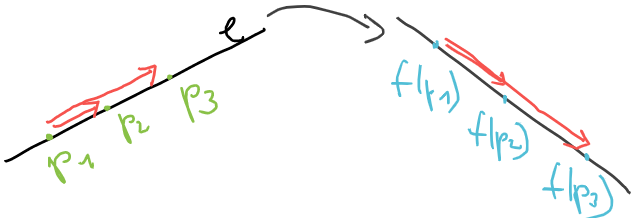
\includegraphics[width=0.5\linewidth]{figures/kollineationen_motivation}
    \label{fig:kollineationen_motivation}
\end{figure}
Dann liegen auch \( f(p_1), f(p_2),f(p_3) \) auf einer Geraden.

\begin{frage*}
    Welche bijektiven Abbildungen \( f\maps X\to X \) haben diese Eigenschaft?
\end{frage*}
\begin{definition*}
    Sei \( X \) ein affiner Raum und \( p_1,p_2,p_3\in X \). Wir nennen \( p_1,p_2,p_3 \) \emph{kollinear}, wenn \( p_1,p_2,p_3 \) auf einer Geraden \( \ell \subset X \) liegen. Wir nennen eine bijektive Abbildung \( f\maps X\to X \) eine Kollineation, falls jede Gerade \( \ell \subset X \) auf eine Gerade \( f(\ell)\subset X \) abgebildet wird.
\end{definition*}
\begin{beispiel}
    Affinitäten
\end{beispiel}
\begin{beispiel}
    Ist \( \affindim-{X}=1 \) und \( f\maps X\to X \) bijektiv, dann ist \( f \) eine Kollineation.
\end{beispiel}
\begin{beispiel}\label{kollinieationen:beispiele:komplexe_konjugation}
    Sei \( X=\complexs^2 \) als affiner Raum über \( \complexs \).
    \begin{align*}
        f\maps \begin{aligned}[t]
            \complexs^2\to \complexs^2\\
            (x,y)&\mapsto &(\explain{\text{komplexe Konjugation}}{\conjugate{x},\conjugate{y          }}).
        \end{aligned}
    \end{align*}
    Dann ist \( f \) eine Kollineation. Das Bild einer Geraden
    \begin{align*}
        (x_0,y_0)+\complexs(x_1,y_1)
    \end{align*}
    ist gegeben durch die Gerade
    \begin{align*}
        (\conjugate{x_0},\conjugate{y_0})+\complexs(\conjugate{x_1},\conjugate{y_1}),
    \end{align*}
    aber \( f \) ist \emph{keine Affinität}!
\end{beispiel}
\begin{bemerkung*}
    Die komplexe Konjugation
    \begin{align*}
        \begin{aligned}[t]
            \complexs&\to \complexs\\
            x&\mapsto \conjugate{x}
        \end{aligned}
    \end{align*}
    ist ein Automorphismus von dem Körper \( \complexs \).
\end{bemerkung*}
% !TEX root = ./Vorlesungsmitschrift AGLA 2.tex  
\lecture{Fr 08.05. 10:15}{}
\begin{definition*}
    Sei \( K \) ein Körper. Wir nennen eine Bijektion \( \alpha\maps K\to K \) einen Automorphismus von \( K \) falls gilt
    \begin{align*}
        \alpha(\lambda+\mu)&=\alpha(\lambda)+\alpha(\mu)\quad \forall \lambda,\mu\in K
        \intertext{und}
        \alpha(\lambda\cdot \mu)&=\alpha(\lambda)\cdot \alpha(\mu)\quad \forall  \lambda,\mu\in K
    \end{align*}
\end{definition*}
\begin{beispiel}
    \begin{align*}
        K=\rationals(\sqrt{2})=\Set{x+y\sqrt{2}|x,y\in\rationals}
    \end{align*}
    ist ein Körper und 
    \begin{align*}
        \alpha\maps \begin{aligned}[t]
            \rationals(\sqrt{2})&\to \rationals(\sqrt{2})\\
            x+y\sqrt{2}&\mapsto x-y\sqrt{2}.
        \end{aligned}
    \end{align*}
\end{beispiel}
\begin{satz}\label{alle_automorphismen_auf_r_identitaet}
    Sei \( \alpha\maps \reals\to \reals \) ein Automorphismus von \( \reals \). Dann gilt \( \alpha=\Id_{\reals} \).
\end{satz}
\begin{proof}
    Sei \( \alpha\maps \reals\to \reals \) ein Automorphismus.
    \begin{proofenumerate}
        \item Dann gilt
        \begin{align*}
            \alpha(0)=\alpha(0+0)=\alpha(0)+\alpha(0),
        \end{align*}
        also \( \alpha(0)=0 \).
        \item Dann gilt
        \begin{align*}
            0=\alpha(0)=\alpha(\lambda-\lambda)=\alpha(\lambda)+\alpha(-\lambda),
        \end{align*}
        also \( \alpha(-\lambda)=-\alpha(\lambda)\logicspace \forall \lambda\in \reals \).
        \item Dann gilt
        \begin{align*}
            \alpha(1)=\alpha(1\cdot 1)=\alpha(1)\alpha(1),
        \end{align*}
        also \( \alpha(1)=1 \) und daher
        \begin{align*}
            \alpha(n)=n\logicspace \forall n\in \wholes,
        \end{align*}
        \zb
        \begin{align*}
            \alpha(2)=\alpha(1+1)=\alpha(1)+\alpha(1)=1+1=2.
        \end{align*}
        \item Sei \( p\in \wholes \), \( q\in \naturals \), dann gilt
        \begin{align*}
            q\alpha\left( \frac{p}{q} \right)\begin{aligned}[t]
                &=\alpha(q)\alpha\left( \frac{p}{q} \right)=\alpha\left( q\frac{p}{q} \right)=\alpha(p)=p,
            \end{aligned}
        \end{align*}
        also \( \alpha\left( \frac{p}{q}=\frac{p}{q} \right) \) oder \( \alpha(t)=t\quad \forall t\in \rationals \).
        \item Sei \( \lambda\in \reals_{>0} \). Dann \texists  \( \mu\in\reals \) mit \( \lambda=\mu^2 \) und
        \begin{align*}
            \alpha(\lambda)=\alpha(\mu^2)=\alpha(\mu)\cdot \alpha(\mu)>0,
        \end{align*}
        also
        \begin{align*}
            \alpha(\lambda)>0\quad \forall \lambda\subset \reals>0.
        \end{align*}
    \end{proofenumerate}
    Wir zeigen nun \( \alpha(\lambda)=\lambda\quad \forall \lambda\in \reals \).

    \minisec{Gegenannahme}
    Sei \( \lambda\in \reals \) mit \( \alpha(\lambda)\neq \lambda \). Wir diskutieren den Fall \( \alpha(\lambda)<\lambda \) (\( \alpha(\lambda)>\lambda \) geht genauso).

    Wähle \( \frac{p}{q}\in \rationals \) mit
    \begin{align*}
        \alpha(\lambda)<\frac{p}{q}<\lambda.
    \end{align*}
    Dann gilt
    \begin{align*}
        \alpha(\lambda-\frac{p}{q})=\alpha(\lambda)-\frac{p}{q}<0
    \end{align*}
    \contra zu \( \lambda-\frac{p}{q}>0 \).
\end{proof}

\subsection*{Eine Familie von Kollineationen}
\begin{idee*}
    Wir verallgemeinern \thref{kollinieationen:beispiele:komplexe_konjugation}, um eine größere Klasse an Kollineationen zu erhalten als Affinitäten.
\end{idee*}
\begin{beispiel}
    \begin{align*}
        f\maps \begin{aligned}[t]
            \complexs^2&\to \complexs^2\\
            (x,y)&\mapsto (\conj{x},\conj{y})
        \end{aligned}
    \end{align*}
    respektiert Addition, \dh
    \begin{align*}
        f(z+z')=f(z)+f(z')\quad \forall z,z'\in \complexs^2,
    \end{align*}
    und hat die Eigenschaft
    \begin{align*}
        f(\lambda z)=\conj{\lambda} f(z)\quad \forall \lambda\in \complexs\logicspace \forall z\in \complexs^2.
    \end{align*}
    \tto Wir nennen \( f \) semilinear.
\end{beispiel}
\begin{definition*}
    Seien \( V,W \) Vektorräume über einem Körper \( K \). Wir nennen eine Abbildung \( F\maps V\to W \) \emph{semilinear}, wenn es einen Automorphismus \( \alpha \) von \( K \) gibt, sodass gilt
    \begin{itemize}
        \item \(F(v+v')=F(v)+F(v')\quad \forall v,v'\in V\)
        \item \( F(\lambda v)=\alpha(\lambda) F(v)\quad \forall \lambda\in K \logicspace \forall v\in V\).
    \end{itemize}
\end{definition*}
\begin{definition*}
    Seien \( X,Y \) affine Räume über einem Körper \( K \). Wir nennen eine Abbildung
    \begin{align*}
        f\maps X\to Y
    \end{align*}
    \emph{semiaffin}, wenn es eine \emph{semilineare Abbildung} \( F\maps T(X)\to T(Y) \) gibt mit
    \begin{align*}
        \vv{f(p) f(q)}=F(\vv{pq})\logicspace \forall p,q\in X.
    \end{align*}
    Falls \( f \) außerdem bijektiv ist, dann nennen wir \( f \) eine Semiaffinität.
\end{definition*}
\begin{lemma}
    Sei \( f\maps X\to X \) eine Semiaffinität eines affinen Raumes \( X \). Dann ist \( f \) eine Kollineation.
\end{lemma}
\begin{proof}[Beweisidee]
    Sei \( \ell \subseteq X \) eine Gerade, \( p_0\in \ell \). Dann ist
    \begin{align*}
        T(\ell)=\Set{\vv{p_0 x}, x\in \ell}\subseteq T(x)
    \end{align*}
    ein \( K \)-Untervektorraum mit
    \begin{align*}
        \dim_K T(\ell)=1.
    \end{align*}
    Sei \( F\maps T(X)\to T(X)  \) die zu \( f \) gehörige semilineare Abbildung.

    Wir betrachten 
    \begin{align*}
        T(f(\ell))
        \begin{aligned}[t]
            &=\Set{\vv{f(p_0) f(x), x\in \ell}}\\
            &=\Set{F(\vv{p_0 x}), x\in \ell}
            &=F(T(\ell)).
        \end{aligned}        
    \end{align*}
    Dann ist auch \( F(T(\ell))\subseteq T(X) \) ein \( \explain{\text{Übung}}{K \text{-Untervektorraum}} \) der Dimension \( 1 \), also
    \begin{align*}
        f(\ell)\subseteq X
    \end{align*}
    eine Gerade.
\end{proof}
\begin{frage*}
    Gibt es Kollineationen, die keine Semiaffinität sind?
\end{frage*}
\tto Ja, \zb für \( \dim X=1 \).
\subsection*{Hauptsatz der affinen Geometrie}

Sei \( K \) ein Körper mit \( \anzahl K\geq 3 \), \( X \) ein affiner Raum über \( K \) mit \( \dim X\geq 2 \) und \( f\maps X\to X \) eine Kollineation. Dann ist \( f \) eine Semiaffinität.

\begin{bemerkung*}
    Aus \thref{alle_automorphismen_auf_r_identitaet} folgt, dass über \( \reals \) jede semilineare Abbildung linear ist.
\end{bemerkung*}
\begin{korollar*}
    Sei \( X \) ein affiner Raum über \( \reals \) mit \( \dim X\geq 2 \), \( f\maps X\to X \) eine Kollineation. Dann ist \( f \) eine Affinität.
\end{korollar*}

\section{Quadriken}
\begin{motivation*}
    Affine Unterräume der \( \reals^n \) sind gegeben durch \emph{lineare} Gleichungssysteme.
\end{motivation*}
\minisec{Jetzt:}
Betrachte den Unterraum im \( \reals^n \), der entsteht als Lösungsmenge einer \emph{quadratischen} Gleichung.
\begin{beispiele*}[im \( \reals^2 \)]
    \begin{enumerate}
        \item der Kreis
        \begin{align*}
            \Set{(x,y)\in \reals^2|x^2+y^2=1}
        \end{align*}
        \item Ellipsen, \( a,b>0 \)
        \begin{align*}
            E=\Set{(x,y)\in \reals^2|ax^2+by^2=1}
        \end{align*}
        \begin{figure}[H]
            \centering
            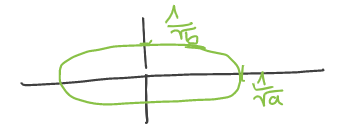
\includegraphics[width=0.5\linewidth]{figures/quadriken_beispiel_ellipse}
            \label{fig:quadriken_beispiel_ellipse}
        \end{figure}
        \item Parabel
        \begin{align*}
            y=ax^2
        \end{align*}
        \begin{figure}[H]
            \centering
            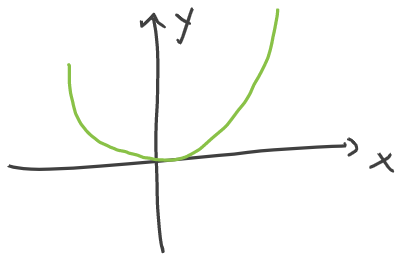
\includegraphics[width=0.5\linewidth]{figures/quadriken_beispiel_parabel}
            \label{fig:quadriken_beispiel_parabel}
        \end{figure}
        \item Hyperbeln, \( a,b>0 \)
        \begin{align*}
            ax^2-by^2=1 
        \end{align*}
        \begin{figure}[H]
            \centering
            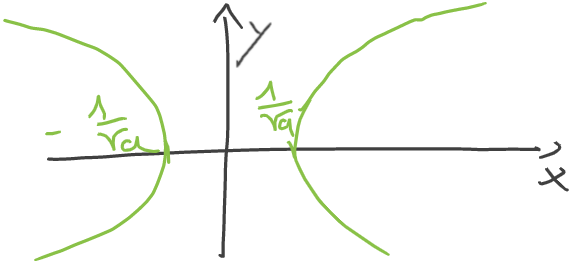
\includegraphics[width=0.5\linewidth]{figures/quadriken_beispiel_hyperbeln}
            \label{fig:quadriken_beispiel_hyperbeln}
        \end{figure}
        \item \( x^2=0 \)
        \begin{figure}[H]
            \centering
            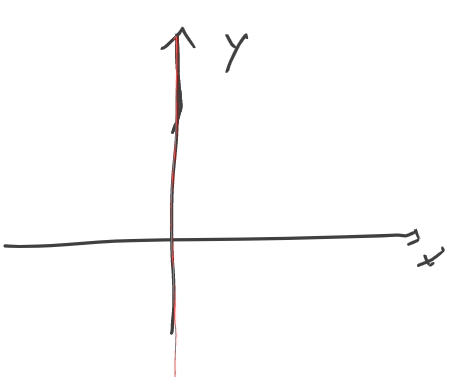
\includegraphics[width=0.4\linewidth]{figures/quadriken_beispiel_y_achse}
            \label{fig:quadriken_beispiel_y_achse}
        \end{figure}
        \item \( xy=0 \)
        \begin{figure}[H]
            \centering
            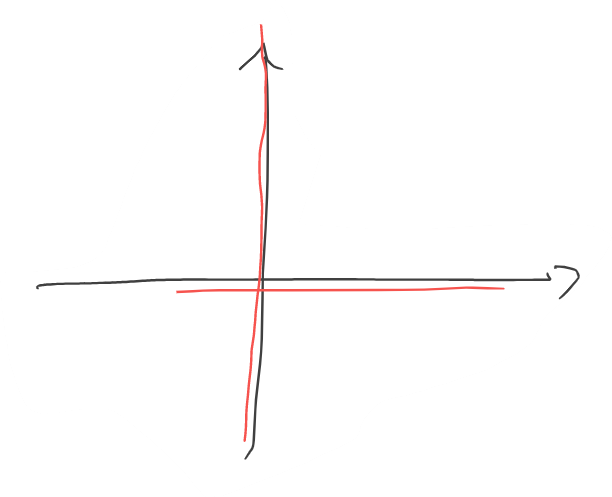
\includegraphics[width=0.4\linewidth]{figures/quadriken_beispiel_x_achse_und_y_achse}
            \label{fig:quadriken_beispiel_x_achse_und_y_achse}
        \end{figure}
        \item \( x^2+y^2=0 \)
        \begin{figure}[H]
            \centering
            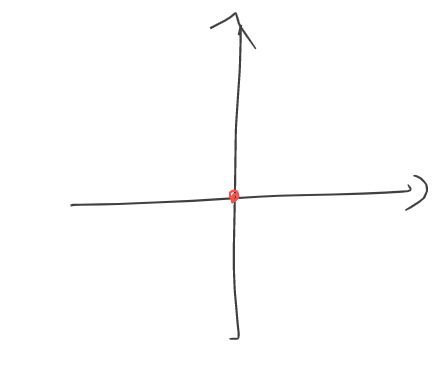
\includegraphics[width=0.4\linewidth]{figures/quadriken_beispiel_ursprung}
            \caption*{Der Ursprung}
            \label{fig:quadriken_beispiel_ursprung}
        \end{figure}
    \end{enumerate}
\end{beispiele*}
\begin{beispiele*}
    Sei \( Q\subseteq \reals^2 \) gegeben durch
    \begin{align*}
        x_1^2+2x_1x_2+2x_2^2+2x_1=0.
    \end{align*}
    Erster Schritt: Entferne den \enquote{gemischten} Term \( x_1 x_2 \).
    \begin{align*}
        (x_1+x_2)^2+x_2^2+2x_1=0.
    \end{align*}
    Nach der Koordinatentransformation
    \begin{align*}
        y_1=x_1+x_2\quad y_2=x_2
    \end{align*}
    ist \( Q \) gegeben durch
    \begin{align*}
        y_1^2+y_2^2+2y_1\cdot 1-2y_2\cdot 1=0.
    \end{align*}
\end{beispiele*}
\begin{bemerkung*}
    Wir können die obigen Gleichungen auch über anderen Körpern \( K \) betrachten, die Lösungsmenge hängt im Allgemeinen wesentlich von \( K \) ab, \zb \( x^2+y^2=0 \).
    \begin{frage*}
        Was passier hier über \( \complexs \), \( \quot{\wholes}{p\wholes} \) für \( p \) prim?
    \end{frage*}
\end{bemerkung*}
\begin{definition*}
    Sei \( K  \) ein Körper. Ein quadratisches Polynom über \( K \) in den Unbestimmten \( x_1,\dotsc, x_n \) ist eine Ausdruck der Form
    \begin{align*}
        P(x_1,\dotsc, x_n)=\sum_{1\leq i, j\leq n} \alpha_{ij}x_i x_j+\sum_{1\leq i\leq n} \alpha_{0i} x_i+\alpha_{00}.
    \end{align*} 
    mit \( \alpha_{ij},\alpha_{0i}, \alpha_{00}\in K \quad \forall 1\leq i,j\leq n \).
\end{definition*}
\begin{bemerkung*}
    Aus einem quadratischen Polynom \( P \) über \( K \) erhält man eine Abbildung
    \begin{align*}
        K^n&\to K\\
        (t_1,\dotsc,t_n)&\mapsto P(t_1,\dotsc,t_n).
    \end{align*}
\end{bemerkung*}
\begin{achtung*}
    Zwei unterschiedliche Polynome \( P_1,P_2 \) müssen nicht notwenigerweise identisch sein, um dieselben Abbildung zu induzieren.
\end{achtung*}
\begin{beispiel*}
    \( K=\mathbb{F}_p=\quot{\wholes}{p\wholes} \). Körper mit \( p \) Elementen mit \( p \) prim, \( n=1 \).
    \begin{align*}
        P_1&=x\\
        P_2&=x^p.
    \end{align*}
    Nach Fermats kleinem Satz gilt
    \begin{align*}
        t\equiv t^p \mod p\quad \forall t\in \quot{\wholes}{p\wholes}.
    \end{align*}
    Für \( p=2 \) sind \( P_1,P_2 \) quadratische Polynome nach obiger Definition.
\end{beispiel*}
\begin{definition*}
    Wir nennen eine Teilmenge \( Q\subseteq K^n \) eine \emph{Quadrik}, falls \( Q \) definiert ist durch
    \begin{align*}
        Q=\Set{(x_1,\dotsc,x_n)\in K^n|P(x_1,\dotsc,x_n)=0}
    \end{align*}
    für ein quadratisches Polynom \( P \) über \( K \).
\end{definition*}
\begin{beispiele*}
    \begin{itemize}
        \item \( x_1^2+\dotsb+x_n^2=0 \) über \( \reals \) ergibt den Ursprung.
        \item \( a_1x_1^2+\dotsb+a_n x_n^2=1 \), \( a_1,\dotsb,a_n>0 \) über \( \reals \) ergibt einen Ellipsoid.
        \item \( K=\reals \), \( P=x_1^2+2x_1x_2+5x_2^2 \). Dann ist
        \begin{align*}
            Q=\Set{x_1,x_2\in \reals^2|\underbrace{(x_1,x_2)\begin{pNiceMatrix} 1 & \underline{1} \\ \underline{1} & 5 \end{pNiceMatrix}\begin{pNiceMatrix} x_1 \\ x_2 \end{pNiceMatrix}=0}_{P(x_1,x_2)}}.
        \end{align*}
    \end{itemize}
\end{beispiele*}
\begin{frage*}
    Wie können wir im Allgemeinen Quadriken in Matrizenschreibweise ausdrücken?
\end{frage*}









% !TEX root = ./Vorlesungsmitschrift AGLA 2.tex  
\lecture{Di 12.05. 10:15}{}
\renewcommand{\transpose}[1]{\leftidx{^t}{#1}{}}
\begin{idee*}
  Sei
  \begin{align*}
    P(x_1,\dotsc,x_n)=\sum\limits_{1\leq i\leq j\leq n}\alpha_{ij}x_i x_j+\sum\limits_{1\leq i \leq n}\alpha_{0i}x_i\cdot 1+\alpha_{00}\cdot 1^2.
  \end{align*}
  Wir schreiben
  \begin{align*}
    x'=\begin{pNiceMatrix} 1\\ x_1 \\ \vdots \\ x_n \end{pNiceMatrix}\in K^{n+1}.
  \end{align*}
  und (sei im Folgenden \( \characteristic K\neq 2 \))
  \begin{align*}
    A=\begin{pNiceArray}{C|CCCC}
      a_{00}& a_{01} & \Cdots & \Cdots & a_{0n} \\
      \hline
      a_{10} & a_{11} & a_{12} & \Cdots & a_{1n} \\
       \Vdots & \Vdots & \Ddots &  & \Vdots \\
       \\
       a_{n0} & a_{n1} & \Cdots & \Cdots & a_{nn}
    \end{pNiceArray}
  \end{align*}
  mit \( a_{ii}=\alpha_{ii}\quad \forall 0\leq i\leq n \).
  \begin{align*}
    a_{ij}=a_{ji}=\frac{1}{2}\alpha_{ij}\text{ für }0\leq i<j\leq n.
  \end{align*}
  Es gilt dann
  \begin{align*}
    P(x_1,\dotsc,x_n)=\transpose{x'}A'x'
  \end{align*}
  und
  \begin{equation*}
    Q=\Set{(x_1,\dotsc,x_n)\in K^n| \transpose{x'}A'x'=0}.
  \end{equation*}
\end{idee*}
\begin{bemerkung*}
  Die Matrix \( A' \) ist symmetrisch (nach Konstruktion).
\end{bemerkung*}
\begin{definition*}
  In obiger Notation nennen wir \( A' \) di erweiterte Matrix zu \( P \) und \( x' \) den erweiterten Spaltenvektor zu \( x \). Wir sagen, dass \( A'\in \Mat_{(n+1)\times(n+1)}(K) \) die Quadrik \( Q \) beschreibt, wenn gilt
  \begin{equation*}
    Q=\Set{x\in K^n|\transpose{x'}A'x'=0}.
  \end{equation*}
\end{definition*}
\begin{notation*}
  Für \( P \) wie oben schreiben wir
  \begin{equation*}
    A=\begin{pNiceMatrix}
      a_{11} & \Cdots & a_{1n} \\
      \Vdots &  & \Vdots \\
      a_{n1} & \Cdots & a_{nn}
    \end{pNiceMatrix}
  \end{equation*}
  für den \enquote{rein quadratischen} Anteil von \( P \).
\end{notation*}
\begin{bemerkung*}
  Sei \( Q\subseteq K^n \) eine Quadrik. Dann gibt es im Allgemeinen nicht nur eine erweiterte Matrix \( A' \) die \( Q \) beschreibt. Ist
  \begin{equation*}
    Q=\Set{(x_1,\dotsc,x_n)\in K^n| \transpose{x'}A'x'=0},
  \end{equation*}
  dann beschreibt auch \( \lambda A' \) mit \( \lambda\in K\setminus\zeroset \) die Quadrik \( Q \).
\end{bemerkung*}
\begin{frage*}
  Wie verhalten sich Quadriken unter Koordinatentransformationen / Affinitäten?
\end{frage*}
\begin{beispiel*}
  \( K=\rationals \). \( P(x_1,x_2)=x_1^2+x_2^2 \).
  \begin{align*}
    \begin{pNiceMatrix} x_1 \\ x_2 \end{pNiceMatrix}&\begin{aligned}[t]
      &=\begin{pNiceMatrix} y_1+y_2 \\ y_2+1 \end{pNiceMatrix}\\
      &=\begin{pNiceMatrix} 1 & 1 \\ 0 & 1 \end{pNiceMatrix}\begin{pNiceMatrix} y_1 \\ y_2 \end{pNiceMatrix}+\begin{pNiceMatrix} 0 \\ 1 \end{pNiceMatrix}.
    \end{aligned}\\
    P(x_1,x_2)&\begin{aligned}[t]
      &=(y_1+y_2)^2+(y_2+1)^2\\
      &=y_1^2+2y_1 y_2+2 y_2^2+2y_2+1
    \end{aligned}
  \end{align*}
  ist wieder ein quadratisches Polynom.
\end{beispiel*}
\begin{lemma}\label{affinitaet_bildet_quadriken_auf_quadriken_ab}
  Sei \( K \) ein Körper mit \( \characteristic K\neq2 \), \( Q\leq K^n \) eine Quadrik und \( f\maps K^n\to K^n \) eine Affinität. Dann ist auch \( f(Q)\subseteq K^n \) eine Quadrik.
\end{lemma}
\begin{proof}
  Sei \( Q \) gegeben durch das quadratische Polynom \( P(x_1,\dotsc, x_n) \), also
  \begin{equation*}
    Q=\Set{(x_1,\dotsc,x_n)\in K^n|P(x_1,\dotsc,x_n)=0}.
  \end{equation*}
  Sei \( A' \) die erweiterte Matrix zu \( P \) und \( x' \) der erweiterte Spaltenvektor zu \( x \). Dann gilt
  \begin{align*}
    Q=\Set{(x_1,\dotsc,x_n\in K^n)|\transpose{x'}A'x'=0}.
  \end{align*}
  Als nächstes beschreibe den durch \( f \) gegebenen Koordinatenwechsel. \( f \) ist eine Affinität, also \texists \( b\in K^n \) und \( S\in \GL_n(K) \) mit
  \begin{equation*}
    \begin{split}
      f\maps K^n&\to K^n\\
      x&\mapsto Sx+b.
    \end{split}
  \end{equation*}
  Sei \( y=f(x) \), schreibe \( y'=\begin{pNiceMatrix} 1 \\ y_1 \\ \Vdots \\ y_n \end{pNiceMatrix} \),
  \begin{equation*}
    S'=\begin{pNiceArray}{C|CCC}
      1 & 0 & \Cdots & 0 \\\hline
      b_1 & \Block{3-3}<\LARGE>{S} &  & \\
      \Vdots & & & \\
      b_n & & &
    \end{pNiceArray}.
  \end{equation*}
  Dann gilt \( y'=S'x' \).
  \begin{bemerkung*}
    \( S' \) ist invertierbar mit inverser Matrix
    \begin{equation*}
      T'=\inv{(S')}=\begin{pNiceArray}{C|CCC}
        1 & 0 & \Cdots & 0 \\\hline
         & \Block{3-3}<\LARGE>{\inv{S}} &  & \\
         -\inv{S}b & & & \\
         & & &
      \end{pNiceArray},
    \end{equation*}
    \dh \( x'=T'y' \).
  \end{bemerkung*}
  Es gilt
  \begin{equation*}
    \begin{split}
      f(Q)&=\Set{f((x_1,\dotsc,x_n))\in K^n| P(x_1,\dotsc,x_n)=0}\\
      &=\Set{y\in K^n| \transpose{x'}A'x'=0}\\
      &=\Set{y\in K^n| \transpose{(T'y')}A'(T'y')=0}\\
      &=\Set{y\in K^n| \transpose{y'}\underbrace{\transpose{T'}A'T'}_{\mathclap{\text{symmetrische Matrix}}}y'=0},
    \end{split}
  \end{equation*}
  also ist \( f(Q) \) eine Quadrik mit
  \begin{equation*}
    P'(y_1,\dotsc, y_n)=\transpose{y'}(\transpose{T'}A'T')y'.
  \end{equation*}
\end{proof}
\begin{bemerkung*}
  Der Beweis von \thref{affinitaet_bildet_quadriken_auf_quadriken_ab} zeigt wie sich eine beschreibende Matrix \( A' \) unter einer Koordinatentransformation ändert.
\end{bemerkung*}
\begin{frage*}
  Sei \( Q \) eine Quadrik beschrieben durch eine erweiterte Matrix \( A' \). Find eine Koordinatentransformation \( f \) der \( K^n \), sodass \( f(Q) \) möglichst \enquote{einfach} beschrieben werden kann.
\end{frage*}
\minisec{zweiter Schritt}
Entferne lineare Terme
\begin{equation*}
  (y_1+1)^2+(y_2-1)^2-2=0.
\end{equation*}
Nach der Koordinatentransformation
\begin{equation*}
  z_1=y_1+1\qquad z_2=y_2-1
\end{equation*}
erhalten wir \( z_1^2+z_2^2=2 \), oder nach skalieren mit \( \sqrt{2} \)
\begin{gather*}
  \sqrt{2}w_1= z_1\qquad \sqrt{2}w_2=z_2\\
  w_1^2+w_2^2=1
\end{gather*}
\begin{figure}[H]
  \centering
  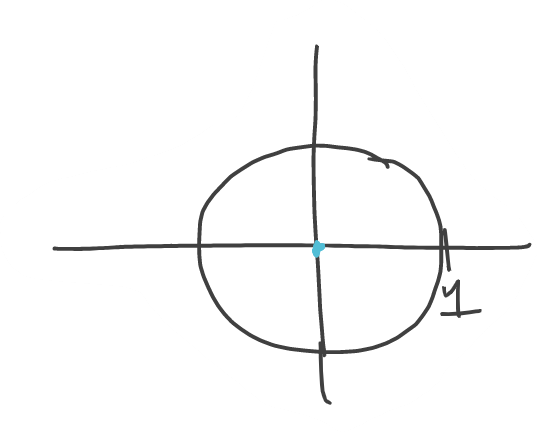
\includegraphics[width=0.5\linewidth]{figures/vereinfachte_quadrik}
  \label{fig:vereinfachte_quadrik}
\end{figure}
\begin{satz}[affine Hauptachsentransformation von reellen Quadriken]\label{affine_hauptachsentranformation_reelle_quadriken}
  Sei \( A'\in \Mat_{(n+1)\times(n+1)}(\reals) \) eine symmetrische Matrix und die Quadrik \( Q\subseteq \reals^n \) gegeben durch
  \begin{equation*}
    Q=\Set{(x_1,\dotsc,x_n)\in \reals^n|\transpose{x'}A'x'=0}.
  \end{equation*}
  Sei \( A \) der rein quadratische Anteil von \( A' \), \( m=\rang A \) und \( m'=\rang A' \). Dann gibt es eine Affinität \( f\maps \reals^n\to \reals^n \), sodass \( f(Q) \) beschrieben wird durch eine der folgenden Gleichungen:
  \begin{eigenschaftenenumerate}
    \item \( m=m' \):
    \begin{equation*}
      y_1^2+\dotsb+y_k^2-y_{k+1}^2-\dotsb-y_m^2=0
    \end{equation*}
    für ein \( 0\leq j \leq m \).
    \item \( m+1=m' \):
    \begin{equation*}
      y_1^2+\dotsb+y_k^2-y_{k+1}^2-\dotsb-y_m^2=1
    \end{equation*}
    für ein \( 0\leq k \leq m \).
    \item \( m+2=m' \):
    \begin{equation*}
      y_1^2+\dotsb+y_k^2-y_{k+1}^2-\dotsb-y_m^2+2_{y_{m+1}}=0
    \end{equation*}
    für ein \( 0\leq k\leq m \).
  \end{eigenschaftenenumerate} 
\end{satz}
\begin{frageuebung}
  Warum gilt immer \( m\leq m'\leq m+2 \)?
\end{frageuebung}
\begin{proof}[Beweis zu \thref{affine_hauptachsentranformation_reelle_quadriken}]
  Sei
  \begin{equation*}
    A'=\begin{pNiceArray}{C|CCC}
      a_{00} & a_{01} & \Cdots & a_{0n} \\\hline
      a_{10} & \Block{3-3}<\LARGE>{A} &  & \\
      \Vdots & & & \\
      a_{n0} & & &
    \end{pNiceArray}.
  \end{equation*}
  mit \( A\in \Mat_{n\times n}(\reals) \).
  \begin{proofenumerate}[label=Schritt \arabic*]
    \item Entferne gemischte Terme.
    \begin{idee*}
      Wollen \( A \) in Diagonalgestalt bringen. 
    \end{idee*}
    AGLA \Romannum{1}: Orthogonalisierungssatz für reelle symmetrische Matrizen.

    Wir erhalten eine invertierbare Matrix \( T_1\in \GL_n(\reals) \) mit
    \begin{equation*}
        \transpose{T_1}AT_1=\begin{pNiceArray}{C|C|C}
            I_k & 0 & 0\\\hline
            0 & -I_{m-k} & 0\\\hline
            0 & 0 & 0
        \end{pNiceArray},
    \end{equation*}
    \( I_l \) Einheitsmatrix der Dimension \( l \), \( m=\rang A \), \( k \) Zahl der positiven Eigenwerte von \( A \) (mit Vielfachheit).

    Sei
    \begin{equation*}
      T_1'=\begin{pNiceArray}{C|CCC}
        1 & 0 & \Cdots & 0 \\\hline
        0 & \Block{3-3}<\LARGE>{T_1} &  & \\
        \Vdots & & & \\
        0 & & &
      \end{pNiceArray}.
    \end{equation*}
    Dann gilt
    \begin{equation*}
      \begin{split}
        A_1'&\definedas \transpose{T_1'}A'T_1'\\
        &=\begin{pNiceArray}{C|CCC}[create-large-nodes]
          c_{00} & c_{01} & \Cdots & c_{0n} \\\hline
          c_{10} & I_k   & 0   &0    \\\cline{2-4}
          \Vdots & 0  & -I_{m-k}   &0 \\\cline{2-4}
          c_{n0} & 0    & 0    & 0
          \CodeAfter
            \tikz \draw (2-2-large.north east) -- (4-2-large.south east);
            \tikz \draw (2-3-large.north east) -- (4-3-large.south east);
        \end{pNiceArray}
      \end{split}
    \end{equation*}
    für \( c_{00}, c_{01}, \dotsc,c_{0n}, c_{1 0},\dotsc, c_{n 0} \in \reals\) mit \( c_{i0}=c_{0i} \) \tforall \( i \). Die durch \( A' \) bestimmte Quadrik ist gegeben durch
    \begin{equation*}
      y_1^2+\dotsb+y_k^2-y_{k+1}^2-\dotsb-y_m^2+2(c_{01}y_1+\dotsb+c_{0n} y_n)+c_{00}=0.
    \end{equation*}
    \item Reduzieren der linearen Terme. Sei
    \begin{equation*}
      T_2'=\begin{pNiceArray}{C|CCCCCCCCC}
        1 & 0 & \Cdots & & & &&&&0 \\\hline
        -c_{10} & 1 & & & &\Block{4-4}<\Large>{0} \\
        \Vdots & &\Ddots \\
        -c_{k 0} \\
        c_{(k+1)0}\\
        \Vdots\\
        c_{m0}&\Block{4-4}<\Large>{0}\\
        0\\
        \Vdots \\
        0 &&&&&&&&&1
      \end{pNiceArray}
    \end{equation*}
    entsprechend dem Basiswechsel
    \begin{equation*}
      y_i=\begin{cases}
        z_i-c_{i0} & 1\leq i \leq k\\
        z_i+c_{i0} & k<i\leq m\\
        z_i &i>m.
      \end{cases}
    \end{equation*}
    Sei
    \begin{equation*}
      \begin{split}
        A_2'&\definedas \transpose{T_2'}A_1'T_2'\\
        &=\begin{pNiceArray}{C|CCCC|CCC}[create-large-nodes]
          d_{00} & 0 & \Cdots & & 0 & c_{0(m+1)} & \Cdots & c_{0 n}\\\hline
          0 & \Block{2-2}<\large>{I_k}\phantom{-IO} & & \Block{2-2}<\large>{0}\phantom{-IOO} & & \Block{4-3}<\LARGE>{0} \\
          \Vdots &&&&&&&\\\cline{2-5}
          & \Block{2-2}<\large>{0}\phantom{-IOO} & & \Block{2-2}<\large>{-I_{m-k}} &&&&\\
          0&&&&&&\\\hline
          c_{(m+1)0} & \Block{3-4}<\LARGE>{0} & & & &\Block{3-3}<\LARGE>{0}\\
          \Vdots&&&&&&&\\
          c_{n 0}&&&&&&&
          \CodeAfter
            \tikz \draw (2-4-block.north west) --  (4-4-block.south west);
        \end{pNiceArray}.
      \end{split}
    \end{equation*}
    Nach der durch \( T_1'T_2' \) beschriebenen Koordinatentransformation ist \( Q \) gegeben durch
    \begin{multline*}
      z_1^2+\dotsb+z_k^2-z_{k+1}^2-\dotsb-z_m^2+2(c_{(m+1)0}z_{m+1}+\dotsb+c_{n0}z_n)+d_{00}.
    \end{multline*}
    \minisec{Fallunterscheidung}
    \begin{eigenschaftenenumerate}
      \item \( d_{00}=c_{(m+1)0}=\dotsb=c_{n0}=0 \).
      \item \( d_{00}\neq 0 \), \( c_{(m+1)0}=\dotsb=c_{n0}=0 \). Nach eventuellem Multiplizieren der Matrix \( A' \) mit \( (-1) \) und Umordnen der Variablen \( z_i \), können wir \( d_{00}<0 \) annehmen.

      Sei \( \lambda=\sqrt{\abs*{d_{00}}} \) und definiere
      \begin{equation*}
        T_3'=\begin{pNiceArray}{C|CCC}
          1 & 0 & \Cdots & 0\\\hline 
          0 & \Block{3-3}{\lambda I_n}\\
          \Vdots \\
          0
        \end{pNiceArray}.
      \end{equation*}
      Wir berechnen
      \begin{equation*}
        A_3'\definedas \transpose{T_3'}A_2'T_3'.
      \end{equation*}
      Dann ist
      \begin{equation*}
        A_3'=\begin{pNiceArray}{C|CCC}[create-large-nodes]
          -\lambda^2 & 0 & \Cdots & 0 \\\hline
          0 & \lambda^2 I_k   & 0   &0    \\\cline{2-4}
          \Vdots & 0  & -\lambda^2 I_{m-k}   &0 \\\cline{2-4}
          0 & 0    & 0    & 0
          \CodeAfter
            \tikz \draw (2-2-large.north east) -- (4-2-large.south east);
            \tikz \draw (2-3-large.north east) -- (4-3-large.south east);
        \end{pNiceArray}.
      \end{equation*}
      Nach der zu \( T_1' t_2' t_3' \) gehörigen Affinität und Division durch \( \lambda^2 \) wird \( Q \) gegeben durch
      \begin{equation*}
        u_1^2+\dotsb+u_k^2-u_{k+1}^2-u_m^2=1.
      \end{equation*}
      \item \( c_{i0}\neq 0 \) für mindestens ein \( m+1\leq i\leq n \). Nach Umordnen der Variablen \( z_i \), \( m+1\leq i \leq n \) können wir annehmen, dass \( c_{(m+1)0}\neq 0 \) gilt. Betrachte die Koordinatentransformation \( u_i=z_i \), \( i\neq m+1. \),
      \begin{equation*}
        2u_{m+1}=2(c_{(m+1)0}z_{m+1}+\dotsb+c_{n0}z_n)+d_{00}.
      \end{equation*}
      Nach dieser Affinität wird \( Q \) beschrieben durch
      \begin{equation*}
        u_1^2+\dotsb+u_k^2-u_{k+1}^2-\dotsb-u_m^2+2u_{m+1}=0.
      \end{equation*}
    \end{eigenschaftenenumerate}
  \end{proofenumerate}
\end{proof}
% !TEX root = ./Vorlesungsmitschrift AGLA 2.tex  
\lecture{Fr 15.05. 10:15}{}
Resultate der affinen Hauptachsentransformation im \( \reals^2 \): \( m=\rang A \), \( m'=\rang A' \).
\begin{eigenschaftenenumerate}
  \item \( m=m' \):
  \begin{proofdescription}
    \item[\( m=m'=0 \):] \( Q \) gegeben durch \( 0=0 \) \tto Ebene \( \reals^2 \).
    \item[\( m=m'=1 \)] \( x_1^2=0 \) \tto \enquote{doppelte} Gerade. 
    \begin{figure}[H]
      \centering
      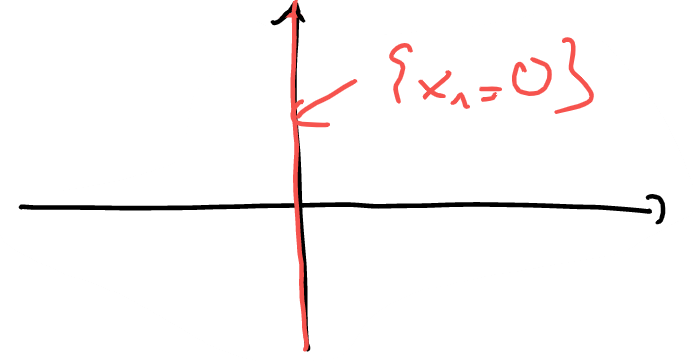
\includegraphics[width=0.5\linewidth]{figures/doppelte_gerade}
      \label{fig:doppelte_gerade}
    \end{figure}
    \item[\( m=m'=2 \)] \( x_1^2+x_2^2=0 \) \tto Punkt.
    \begin{figure}[H]
      \centering
      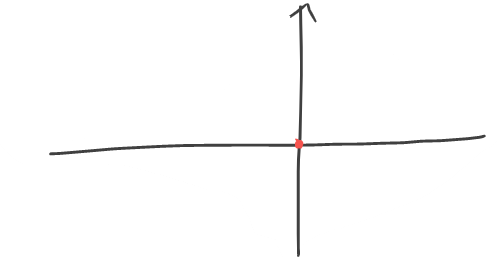
\includegraphics[width=0.5\linewidth]{figures/punkt_quadrik}
      \label{fig:punkt_quadrik}
    \end{figure}
    \item[\( \equalto{(x_1+x_2)(x_1-x_2)}{x_1^2-x_2^2}=0 \)] \tto 2 Geraden.
    \begin{figure}[H]
      \centering
      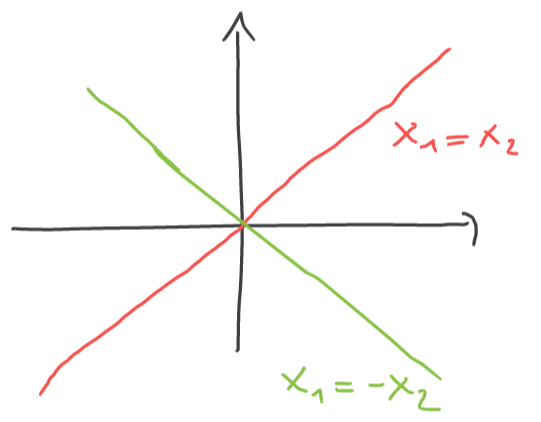
\includegraphics[width=0.5\linewidth]{figures/zwei_geraden_quadrik}
      \label{fig:zwei_geraden_quadrik}
    \end{figure}
  \end{proofdescription}
  \item \( m'=m+1 \).
  \begin{proofdescription}
    \item[\( m=0 \)] \tto \( 0=1 \)  \tto leere Menge.
    \item[\( m=1 \)] \begin{proofdescription}
      \item[\( x_1^2=1 \)]  \tto 2 parallele Geraden
      \begin{figure}[H]
        \centering
        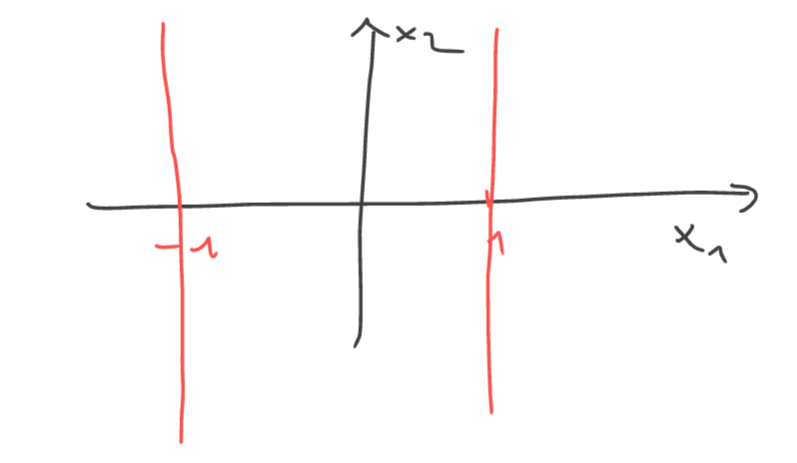
\includegraphics[width=0.5\linewidth]{figures/parallele_geraden_quadrik}
        \label{fig:parallele_geraden_quadrik}
      \end{figure}
      \item[\( -x_1^2=1 \)] \tto leere Menge.
    \end{proofdescription}
    \item[\( m=2 \)] \begin{proofdescription}
      \item[\( -x_1^2-x_2^2=1 \)] \tto \( \emptyset \).
      \item[\( x_1^2-x_2^2=1 \)] \tto Hyperbel. 
      \begin{figure}[H]
        \centering
        \includegraphics[width=0.5\linewidth]{figures/hyperbel_quadrik}
        \label{fig:hyperbel_quadrik}
      \end{figure}
      \item[\( x_1^2+x_2^2=1 \)] \tto Kreis.
      \begin{figure}[H]
        \centering
        \includegraphics[width=0.5\linewidth]{figures/ellipse_kreis_quadrik}
        \label{fig:ellipse_kreis_quadrik }
      \end{figure}
    \end{proofdescription}
    \item \( m'=m+2 \). \begin{proofdescription}
      \item[\( m=0 \)] \begin{proofdescription}
        \item[\( 2x_1=0 \)] \tto Gerade.
      \end{proofdescription}
      \item[\( m=1 \)] \begin{proofdescription}
        \item[\( x_1^2+2x_2=0 \)] \tto Parabel.
        \begin{figure}[H]
          \centering
          \includegraphics[width=0.5\linewidth]{figures/parabel_quadrik}
          \label{fig:parabel_quadrik}
        \end{figure}
      \end{proofdescription}
    \end{proofdescription}
  \end{proofdescription}
\end{eigenschaftenenumerate}
\begin{bemerkung*}
  Verschiedene dieser quadratischen Formen können als \emph{Menge} die gleiche Quadrik \( Q\subseteq \reals^2 \) beschreiben.
\end{bemerkung*}
\begin{beispiel*}
  \begin{equation*}
    \Set{(x_1,x_2)\in \reals^2|x_1^2=0}=\Set{(x_1,x_2)\subset \reals^2| 2x_1=0}.
  \end{equation*}
\end{beispiel*}
\begin{definition*}
  Wir nennen zwei Quadriken \( Q_1,Q_2\subseteq \reals^n \) \emph{geometrisch äquivalent} wenn es eine Affinität \( f\maps \reals^n\to \reals^n \) gibt mit \( f(Q_1)=Q_2 \).
\end{definition*}
\begin{frage*}
  Klassifikation aller Quadriken über \( \reals \) bis auf geometrische Äquivalenz?
\end{frage*}
Für eine Matrix \( B\in \matrices{n}{n}{\reals} \) sei \( \signature{B}=\anzahl-{} \) positive Eigenwerte von \( B \) \( -\anzahl-{} \) negative Eingenwerte von \( B \) die Signatur von \( B \).
\begin{satz}[Geometischer Klassifikationssatz (ohne Beweis)]
  Seien \( Q_1,Q_2\subset \reals^n \) nichtleere Quadriken, die beschrieben werden durch erweiterte Matrizen \( A_1',,A_2' \) mit rein quadratischen Anteilen \( A_1,A_2 \). Seien \( Q_1,Q_2 \) nicht gleich an Hyperebenen.

  Dann sind \( Q_1 \) und \( Q_2 \) \emph{geometrisch äquivalent} \gdw gilt
\begin{align*}
  \rang-{A_1}&=\rang-{A_2},\\
  \rang-{A_1'}&=\rang-{A_2'},\\
  \abs*{\signature-{A_1}}&=\abs*{\signature-{A_2}}\text{ und}\\
  \abs*{\signature-{A_1'}}&=\abs*{\signature-{A_2'}}.
\end{align*}
\end{satz}
\begin{folgerung}
  Sei \( Q\subset \reals^n \) eine nichtleere Quadrik. Dann ist \( Q \) geometrisch äquivalent zu genau einer der folgenden Quadriken.
  \begin{eigenschaftenenumerate}
    \item \label{quadriken_gleich_null_nur_quadrate}\( x_1^2+\dotsb+x_k^2-x_{k+1}^2-\dotsb-x_m^2=0 \), \( 0\leq k\leq m \), \( 2k-m\geq 0 \).
    \item \label{quadriken_gleich_eins}\( x_1^2+\dotsb+x_k^2-x_{k+1}^2-\dotsb-x_n^2=1 \), \( 1\leq k\leq m \).
    \item \label{qadriken_gleich_null_plus_ein_linearer}\( x_1^2+\dotsb+x_k^2-x_{k+1}-\dotsb-x_m^2+2x_{m+1}=0 \), \( 1\leq k\leq m \) und \( 2k-m\geq 0 \).
  \end{eigenschaftenenumerate}
\end{folgerung}
\begin{beispiele*}[Quadriken im \( \reals^3 \)]
  \begin{description}
    \item[Typ \ref{quadriken_gleich_null_nur_quadrate}] \( x_1^2+x_2^2-x_3^2=0 \)
    \begin{figure}[H]
      \centering
      \includegraphics[width=0.5\linewidth]{figures/quadriken_beispiel_kegel}
      \caption*{Kegel}
      \label{fig:quadriken_beispiel_kegel}
    \end{figure}
    \item[Typ \ref{quadriken_gleich_eins}] \begin{itemize}
      \item \( x_1^2+x_2^2=1 \).
      \begin{figure}[H]
        \centering
        \includegraphics[width=0.5\linewidth]{figures/quadriken_beispiel_kreiszylinder}
        \caption*{Kreiszylinder}
        \label{fig:quadriken_beispiel_kreiszylinder}
      \end{figure}
      \item \( x_1^2+x_2^2+x_3^2=1 \).
      \begin{figure}[H]
        \centering
        \includegraphics[width=0.5\linewidth]{figures/quadriken_beispiel_kugel}
        \caption*{Kugel}
        \label{fig:quadriken_beispiel_kugel}
      \end{figure}
      \item \( x_1^2-x_2^2+x_3^2=1 \).
      \begin{figure}[H]
        \centering
        \includegraphics[width=0.5\linewidth]{figures/quadriken_beispiel_zweischaliges_hyperboloid}
        \caption*{Zweischaliges Hyperboloid}
        \label{fig:quadriken_beispiel_zweischaliges_hyperboloid}
      \end{figure}
      \item \( x_1^2+x_2^2-x_3^2=1 \)
      \begin{figure}[H]
        \centering
        \includegraphics[width=0.5\linewidth]{figures/quadriken_beispiel_einschaliges_hyperboloid}
        \caption*{Einschaliges Hyperboloid}
        \label{fig:quadriken_beispiel_einschaliges_hyperboloid}
      \end{figure}
    \end{itemize}
    \item[Typ \ref{qadriken_gleich_null_plus_ein_linearer}] \( x_1^2+x_2^2+2x_3=0 \).
    \begin{figure}[H]
      \centering
      \includegraphics[width=0.5\linewidth]{figures/quadriken_beispiel_elliptisches_paraboloid}
      \caption*{Elliptisches Paraboloid}
      \label{fig:quadriken_beispiel_elliptisches_paraboloid}
    \end{figure}
  \end{description}
\end{beispiele*}
\file{Euklidische affine Räume}
\section{Euklidische affine Räume}
In einem allgemeinen affinen Raum \( X \) haben wir den Begriff von Gerade und parallelen Geraden (Sind \( L,L'\subset X \) Geraden, dann sagen wir, dass \( L \) und \( L' \) parallel sind, falls \( T(L)=T(L') \)).
\begin{figure}[H]
  \centering
  \includegraphics[width=0.5\linewidth]{figures/affine_geraden_lagebeziehungen}
  \label{fig:affine_geraden_lagebeziehungen}
\end{figure}
\begin{frage*}
  Können wir auch \enquote{Winkel} messen zischen zwei sich schneidenden Geraden?
\end{frage*}
\begin{erinnerung*}
  Sei \( V \) ein \( \reals \)-Vektorraum. Ein Skalarprodukt auf \( V \) ist eine \emph{positiv-definite symmetrische Bilinearform}
  \begin{equation*}
    S\maps V\times V\to \reals.
  \end{equation*}
\end{erinnerung*}
\begin{definition*}
  Ein euklidischer affiner Raum ist ein reeller affiner Raum \( (X,T(X),\tau) \) zusammen mit einem Skalarprodukt
  \begin{equation*}
    \scalarproduct{\cdot}{\cdot}\maps T(X)\times T(X)\to \reals
  \end{equation*}
  auf dem Translationsvektorraum \( T(X) \).
\end{definition*}
\begin{beispiel}
  Der \( \reals^n \) als reeller affiner Raum mit dem Standard-Skalarprodukt
  \begin{equation*}
    \begin{split}
      \scalarproduct{\cdot}{\cdot}\maps \underrelate{\vertrelation{\simeq}}{\reals^n}{T(X)}\times \underrelate{\vertrelation{\simeq}}{\reals^n}{T(X)}&\to \reals\\
      (x_1,\dotsc,x_n)\times (y_1,\dotsc,y_n)&\mapsto \sum_{i=1}^{n}x_i y_i.
    \end{split}
  \end{equation*}
\end{beispiel}
\begin{beispiel}
  Die Lösungsmenge \( L \) im \( \reals^n \) eines Systems von linearen Gleichungen \( Ax=b \), \( A\in \matrices{m }{n}{\reals} \), \( b\in \reals^m \)
  \begin{figure}[H]
    \centering
    \includegraphics[width=0.5\linewidth]{figures/hyperebene_beispiel_euklidischer_affiner_raum}
    \label{fig:hyperebene_beispiel_euklidischer_affiner_raum}
  \end{figure}
  mit dem aus dem \( \reals^n \) induzierten Standard-Skalarprodukt auf \( T(L)\explain{\text{Untervektorraum}}{\untervektorraum}\reals^n \)
  \begin{equation*}
    \scalarproduct{\cdot}{\cdot}\maps \begin{aligned}[t]
      T(L)\times T(L)&\to \reals\\
      (x,y) &\mapsto \scalarproduct{x}{y}.
    \end{aligned}
  \end{equation*}
\end{beispiel}
\begin{frage*}
  Definition von Abständen / Winkeln in einem euklidischen affinen Raum?
\end{frage*}
\begin{definition}
  Sei \( X \) ein euklidischer affiner Raum. Wir definieren eine Normabbildung
  \begin{equation*}
    \norm*{\cdot}\maps \begin{aligned}[t]
      T(X)&\to \reals_{\geq 0}\\
      t&\mapsto \norm*{t}\definedas \sqrt{\scalarproduct{t}{t}}
    \end{aligned}
  \end{equation*}
  und eine Metrik
  \begin{equation*}
    d\maps \begin{aligned}[t]
      X\times X&\to \reals_{\geq 0}\\
      (p,q)\mapsto \distance{p}{q}\definedas \norm*{\vv{pq}}.
    \end{aligned}
  \end{equation*}
  \begin{figure}[H]
    \centering
    \includegraphics[width=0.2\linewidth]{figures/metrik_auf_affinem_raum_visualisierung}
    \label{fig:metrik_auf_affinem_raum_visualisierung}
  \end{figure}
\end{definition}
\begin{bemerkung*}
  \( \norm*{\cdot} \) ist eine Norm, da \( \scalarproduct{\cdot}{\cdot} \) ein Skalarprodukt ist. Man kann nachrechnen, dass \( d \) tatsächlich eine Metrik auf \( X \) ist, \zb
  \begin{equation*}
    \distance{p}{q}=\norm*{\vv{pq}}=\norm*{-\vv{qp}}=\abs*{-1}\cdot\vv{qp}=\distance{q}{p}.
  \end{equation*}
\end{bemerkung*}
\begin{definition*}
  Sei \( X \) ein euklidischer affiner Raum, \( p,q,q'\in X \) mit \( p\neq q \), \( q' \), \( L=p\vee q \), \( L'=p\vee q' \).
  \begin{figure}[H]
    \centering
    \includegraphics[width=0.5\linewidth]{figures/affiner_winkel_definition}
    \label{fig:affiner_winkel_definition}
  \end{figure}
  Wir definieren den Winkel \( \lineangle{L}{L'} \) zwischen den Geraden \( L,L' \) durch
  \begin{equation*}
    \lineangle{L}{L'}=\arccos \frac{\abs*{\scalarproduct{\vv{pq}}{\vv{pq'}}}}{\norm*{\vv{pq}}\cdot\norm*{\vv{pq'}}}\in \interval{0}{\frac{\pi}{2}}.
  \end{equation*}
  \begin{figure}[H]
    \centering
    \includegraphics[width=0.3\linewidth]{figures/affiner_winkel_definition_wertebereich}
    \label{fig:affiner_winkel_definition_wertebereich}
  \end{figure}
  \begin{figure}[H]
    \centering
    \includegraphics[width=0.1\linewidth]{figures/affiner_winkel_definition_wertebereich_beispiel}
    \label{fig:affiner_winkel_definition_wertebereich_beispiel}
  \end{figure}
\end{definition*}
\begin{bemerkung*}
  Die Definition des Winkels \( \lineangle{L}{L'} \) ist unabhängig von der Wahl der Elemente \( q,q' \) (solange \( p\neq q,q' \)).
\end{bemerkung*}
% End of lectures

\end{document}
